\documentclass[dvipsnames,twocolumn]{scrartcl}

\usepackage{multicol}
\usepackage{tikz}
\usetikzlibrary{positioning}
\usepackage{pgfplots}
\usepackage{hyperref}
\usepackage{xcolor}
\hypersetup{
	colorlinks,
	linkcolor={red!50!black},
	citecolor={blue!50!black},
	urlcolor={blue!80!black}
}
\usepackage{amsmath}
\usepackage{amssymb}
\usepackage{listings}
\usepackage{cancel}
\usepackage{nicefrac}
\usepackage{esvect}
\usepackage[autostyle]{csquotes}
\usepackage[utf8]{inputenc}
\usepackage{cite}
\usepackage{url}
\usepackage[numbers, sort]{natbib}
\bibliographystyle{alpha}
\lstset{mathescape=true,language=Python}
\providecommand*{\listingautorefname}{Listing}
\lstnewenvironment{algorithm}[1][]
{   
	\lstset{
		mathescape=true,
		frame=tB,
		numbers=left, 
		basicstyle=\scriptsize, 
		keywordstyle=\color{black}\bfseries\em,
		keywords={,input, output, return, datatype, function, in, if, else, foreach, while, begin, end, }
		numbers=left,
		xleftmargin=.04\textwidth,
		#1
	}
}
{}

%opening
\title{Training Deep Models}
\subtitle{General Optimization techniques}
\author{Moritz~Kirschte, INF103333}

\date{Summer Seminar, 06-05-2018}

\begin{document}
	
	\maketitle
	
	\begin{abstract}
		
		My seminar work in the summer semester 18' supervised by \textsc{Prof. Dr. D. Säring} goes about Optimization in Deep Machine Learning. Being a part of such a huge seminar offers me and the other attendees the ability to focus on a specific topic in the complex field of Machine Learning, rather than wasting time and losing details by giving just short overviews. Basic understandings of Linear Algebra and Machine Learning techniques as e.\,g. presented in the first part of the \textsc{DeepLearningBook} by \textsc{Goodfellow et. al}~\cite{Goodfellow-et-al-2016}, namely knowing how to build, code and train a (Deep) Neural Network, is a requirement of this paper. I decided to explicitly announce this target group restriction, to be more focused on very advanced and complex Optimization techniques. As the projects payoff goes hand in hand with the ability to train fast on big machines e.\,g. the \textsc{NVIDIA DGX-II}~\cite{nvidia-dgx-ii}, a few thoughts on optimization techniques seems to be well-suited.\\ I will start with introducing some advanced learning techniques, afterward stay on a powerful normalization thinking in every layer of your neural network and finally conclude with an extra and not usually mentioned chapter when talking about optimization techniques called feature optimization. After reading this paper, you should be fully aware of the most important advanced optimization techniques and you are able to train your model much faster.
		
	\end{abstract}
	
	\tableofcontents
	
	\section{Motivation}
	
	Before introducing first optimizations, a short moment of breath holding is appropriated.
	
	It'll be a Sisyphean task in convincing you to invest time in optimization if you're not able to realize its need. The \textsc{CIFAR-10} dataset is a perfect example of concurrently visualize the progress. In the beginning, we won't be able to take our Deep Neural Network seriously, but after enhancing the Base-AI written in \textsc{Python} chapter by chapter, advancement will be self-evident.
	
	\subsection{Example: CIFAR-10}
	
	CIFAR-10~\cite{cifar-10}, created by \textsc{Alex Krizhevsky}, \textsc{Vinod Nair}, and \textsc{Geoffrey Hinton}, is a benchmark task for object recognition using 32x32 downsampled color hand-labeled images of 10 different object classes: \emph{airplanes, cars, birds, cats, deer, dogs, frogs, horses, ships, and trucks}. It is divided into 50,000 training images and 10,000 test images.
	
	Even modern AI algorithms are not well performing on this dataset (currently round about 2\,\% error rate), so it isn't as simple as an XOR-prediction, for which even a simple Logistic Regression model fits perfectly. Furthermore, you are able to visualize the error easier than with non-visual data.
	
	\begin{figure}
		\caption{CIFAR-10 dataset: Bird ($y=2$)}
		\includegraphics[width=0.2\columnwidth]{sampleImg/bird1}%
		\includegraphics[width=0.2\columnwidth]{sampleImg/bird2}%
		\includegraphics[width=0.2\columnwidth]{sampleImg/bird3}%
		\includegraphics[width=0.2\columnwidth]{sampleImg/bird4}%
		\includegraphics[width=0.2\columnwidth]{sampleImg/bird5}\\%
		\includegraphics[width=0.2\columnwidth]{sampleImg/bird6}%
		\includegraphics[width=0.2\columnwidth]{sampleImg/bird7}%
		\includegraphics[width=0.2\columnwidth]{sampleImg/bird8}%
		\includegraphics[width=0.2\columnwidth]{sampleImg/bird9}%
		\includegraphics[width=0.2\columnwidth]{sampleImg/bird10}
	\end{figure}
	
	\subsection{Problem-Description}
	
	Everybody should be familiar with Moore's law claiming that every 18 to 24 month the number of transistors on ones chip gets doubled.
	
	But according to Wirth's law~\cite{wirth}, who attributed the saying to \textsc{Martin Reiser}: ``The hope is that the progress in hardware will cure all software ills. However, a critical observer may observe that software manages to outgrow hardware in size and sluggishness.', software getting slower more rapidly than hardware becomes faster.
	
	At the time optimization isn't well integrated with the program, the first results of this first intuition aren't promising. After $3,000$ iterations and half an hour of computation time with only using $10,000$ instead of $50,000$ low-resolution images in a logistic regression (1-Layer) NN, results of $41$\,\% accuracy in the train set and $38$\,\% in the test set are present.
	
	Concluding: Simply trust our computational power more than our brain might not be a good idea for Deep-NNs.
	
	\begin{figure}
		\caption{Performance comparison of Neural-Networks of different Deepness}
		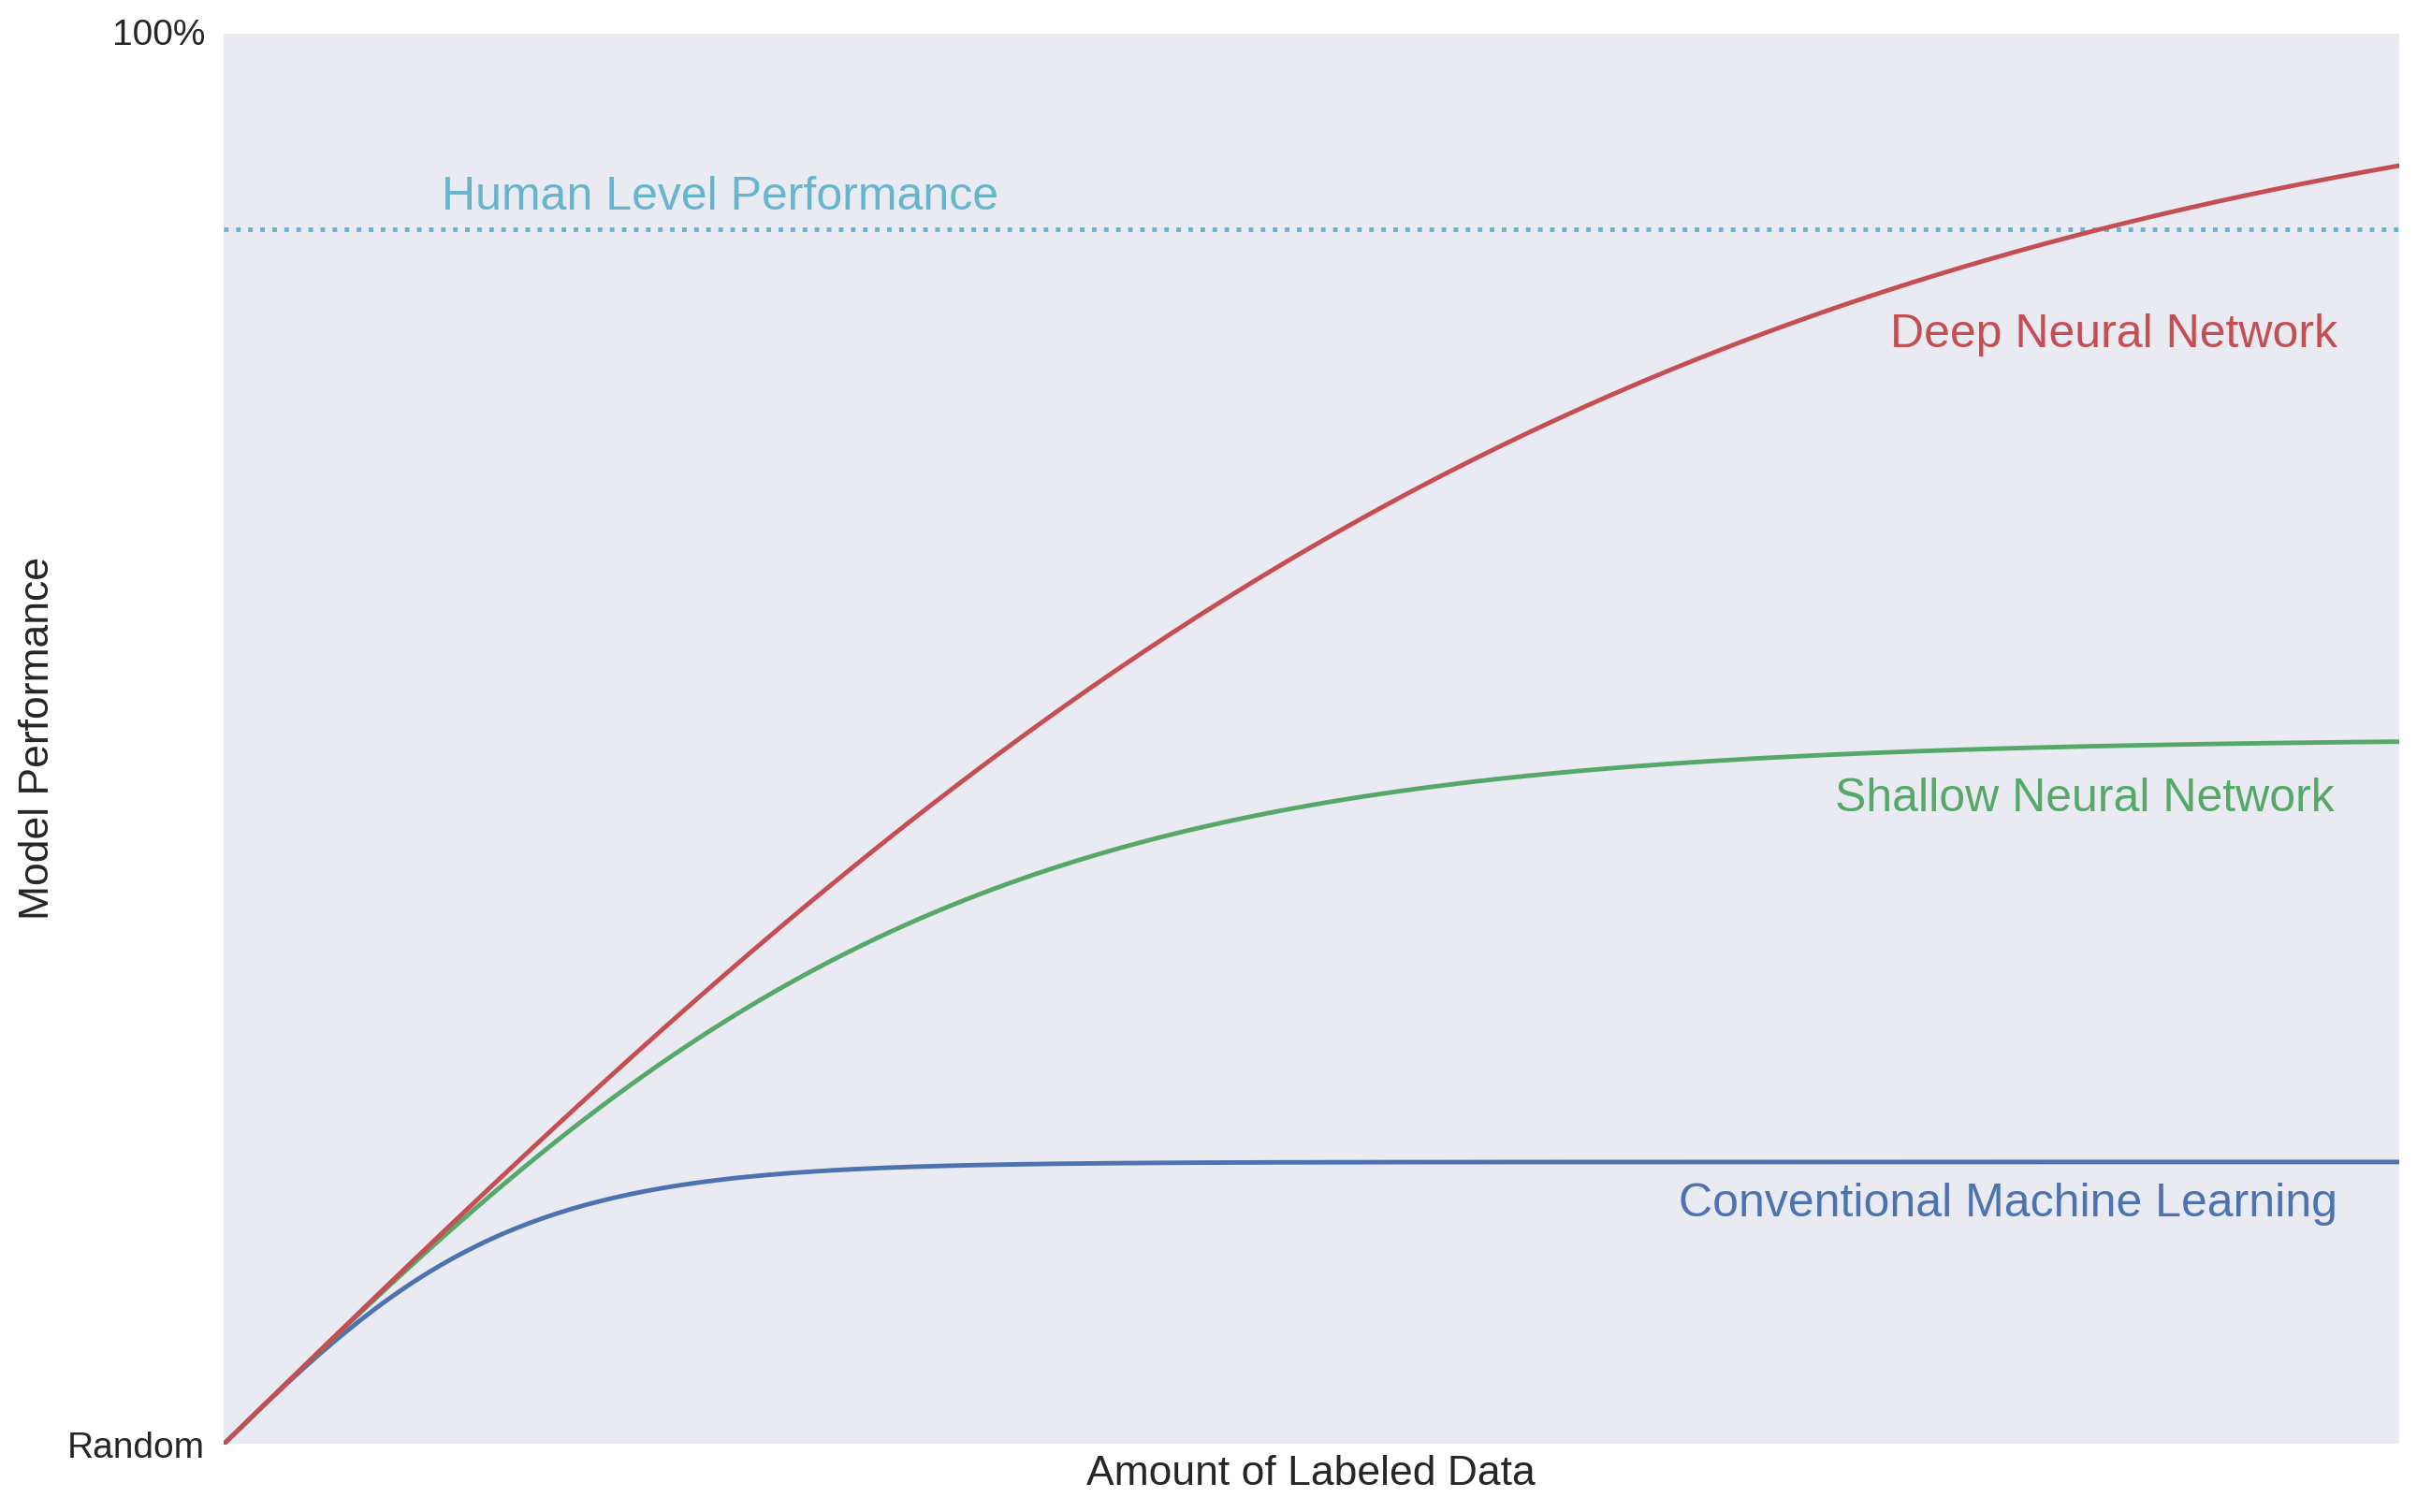
\includegraphics[width=\columnwidth]{data_size_vs_model_performance_v2}%
		%Useful: https://lilianweng.github.io/lil-log/2017/06/21/an-overview-of-deep-learning.html
	\end{figure}
	
	And good model performance comes only from deep and large Neural Networks.
	
	%%%%%%%%%%%%%%%%%%%%%%%%%%%%%%%%%%%%%%%%%%%%%%%%%%%%%%%%%%%%%
	
	\section{Optimizer}
	
	The first topic, I want to present addresses directly the performance improvement. Deciding to start with this topic is not caused by actual relevance to the accuracy as regularization does, it's because building a house on sand rather than solid rock is not a good idea.
	
	\subsection{Batch Gradient Descent}
	
	Given a multi-dimensional function ${\cal F}(x)$ Gradient Descent takes an estimate for any input $a_i$ on how to change the parameter $a$ best to get a smaller function value ${\cal F}(a_{i+1})$ using the fact, that ${\cal F}(x)$ decreases fastest if one goes from $a$ in the direction of the (negative) gradient at $a$: $-\nabla {\cal F}(a)$:
	\begin{itemize}
		\item guess $x_0$
		\item calculate next ($n \ge 0$): $x_{n+1} = x_n - \gamma_n \nabla {\cal F}(x_n)$
		\item hopefully convergence: ${\cal F}(x_0) \ge {\cal F}(x_1) \ge {\cal F}(x_2) \ge \dots$
	\end{itemize}
	
	You have to choose the \emph{learning rate} $\gamma$ carefully, because too big step sizes diverge and too small step sizes take too long per iteration but can reach a better estimate after reaching the region of convergence. A thoughtful combination would also be to introduce \emph{learning rate decay} with a second parameter $\beta$ affecting how much the learning rate will decay at the next total iteration step size in order to be fast at the beginning and slower and more precise at the end. Problematic on Gradient Descent is additionally, that there is a potential to get stuck in a suboptimal local minimum missing the global minimum, but even in higher dimensional spaces, such local minimums are very rare, because it has to be in every dimension a minimum. If not, it'll be a saddle-node and there is even one last direction to move onto. Some kinds of neural networks like e.\,g. logistic regression can guarantee, that they have only one minimum.\\
	
	The way how to implement Gradient Descent in a Neural Network is described in the following algorithm.\\
	Given the weights on each layer $l$ $W^{[l]} \text{ and } b^{[l]}$, the training matrices $(X \in \mathbb{R}^{n,m}, Y \in \mathbb{R}^{1,m})$ and the learning rate, also called step size, $\alpha$:
	\begin{lstlisting}[frame=single,caption={Batch Gradient Descent Algorithm}]
forward_prop(Input ${\cal X}$,
   Weight ${\cal W}^{[l]}$, Bias $b^{[l]}$)
Costs ${\cal J}$ $\gets$ $\frac{1}{\color{red}{m}} \times \sum_{i=1}^{\color{red}{m}}{\cal L}oss(\hat{y^{(i)}},y^{(i)})$
back_prop(${\cal A}^{[L]} = \hat{{\cal Y}}$, Output ${\cal Y}$)
${\cal W}^{[l]} \gets {\cal W}^{[l]} - \alpha\times d{\cal W}^{[l]}$
$b^{[l]} \gets b^{[l]} - \alpha\times db^{[l]}$
	\end{lstlisting}
	These steps are repeated as long as a certain cost is reached or a random number of steps is taken.
	
	The overall problem of \emph{Gradient Descent} is, that performance issues are basically lying on $m$ partly-redundant training examples (e.g. $320,000,000$ US-citizens). The next step of gradient descent can only be done after summing up over all $m$ training examples ignoring the fact, that some of the training examples might be redundant and even the first $1$\,\% offer a quite good estimate of the right direction.
	
	\subsection{Stochastic GD (SGD)}
	
	\emph{Stochastic Gradient Descent (SDG)} directly addresses this problem of \emph{Gradient Descent} by calculating the loss and updating the gradients every $i^{th}$ training example. One step towards all training examples is called an \emph{epoch}. It's important to note, that shuffling the data before applying \emph{Stochastic Gradient Descent} is important, so that our AI doesn't learn something about the order of how we feed in the examples.
	
	But sadly, this technique adds a lot of noise and even towards the minimum it dither back and forth without any convergence. Secondly, the per iteration performance trickles down significantly, due to the missing vectorization possibilities offering parallelism afforded by modern computing platforms.
	
	\begin{lstlisting}[frame=single,caption={Stocastic Gradient Descent Algorithm}]
$\color{orange}shuffle([{\cal X}, {\cal Y}])$
for t in range(1,m):
   forward_prop(Input ${\cal X}^{(t)}$,
      Weight ${\cal W}^{[l]}$, Bias $b^{[l]}$)
   Costs ${\cal J}$ $\gets$ $\color{orange}{\cal L}oss(\hat{y^{(t)}},y^{(t)})$
   back_prop(${\cal A}^{[L](t)} = \hat{y^{(t)}}$, Output $y^{(t)}$)
   ${\cal W}^{[l]} \gets {\cal W}^{[l]} - \alpha\times d{\cal W}^{[l]}$
   $b^{[l]} \gets b^{[l]} - \alpha\times db^{[l]}$
	\end{lstlisting}
	
	\begin{figure}
		\caption{Noise behavior in different GD-algorithms visualized on a contour plot}
		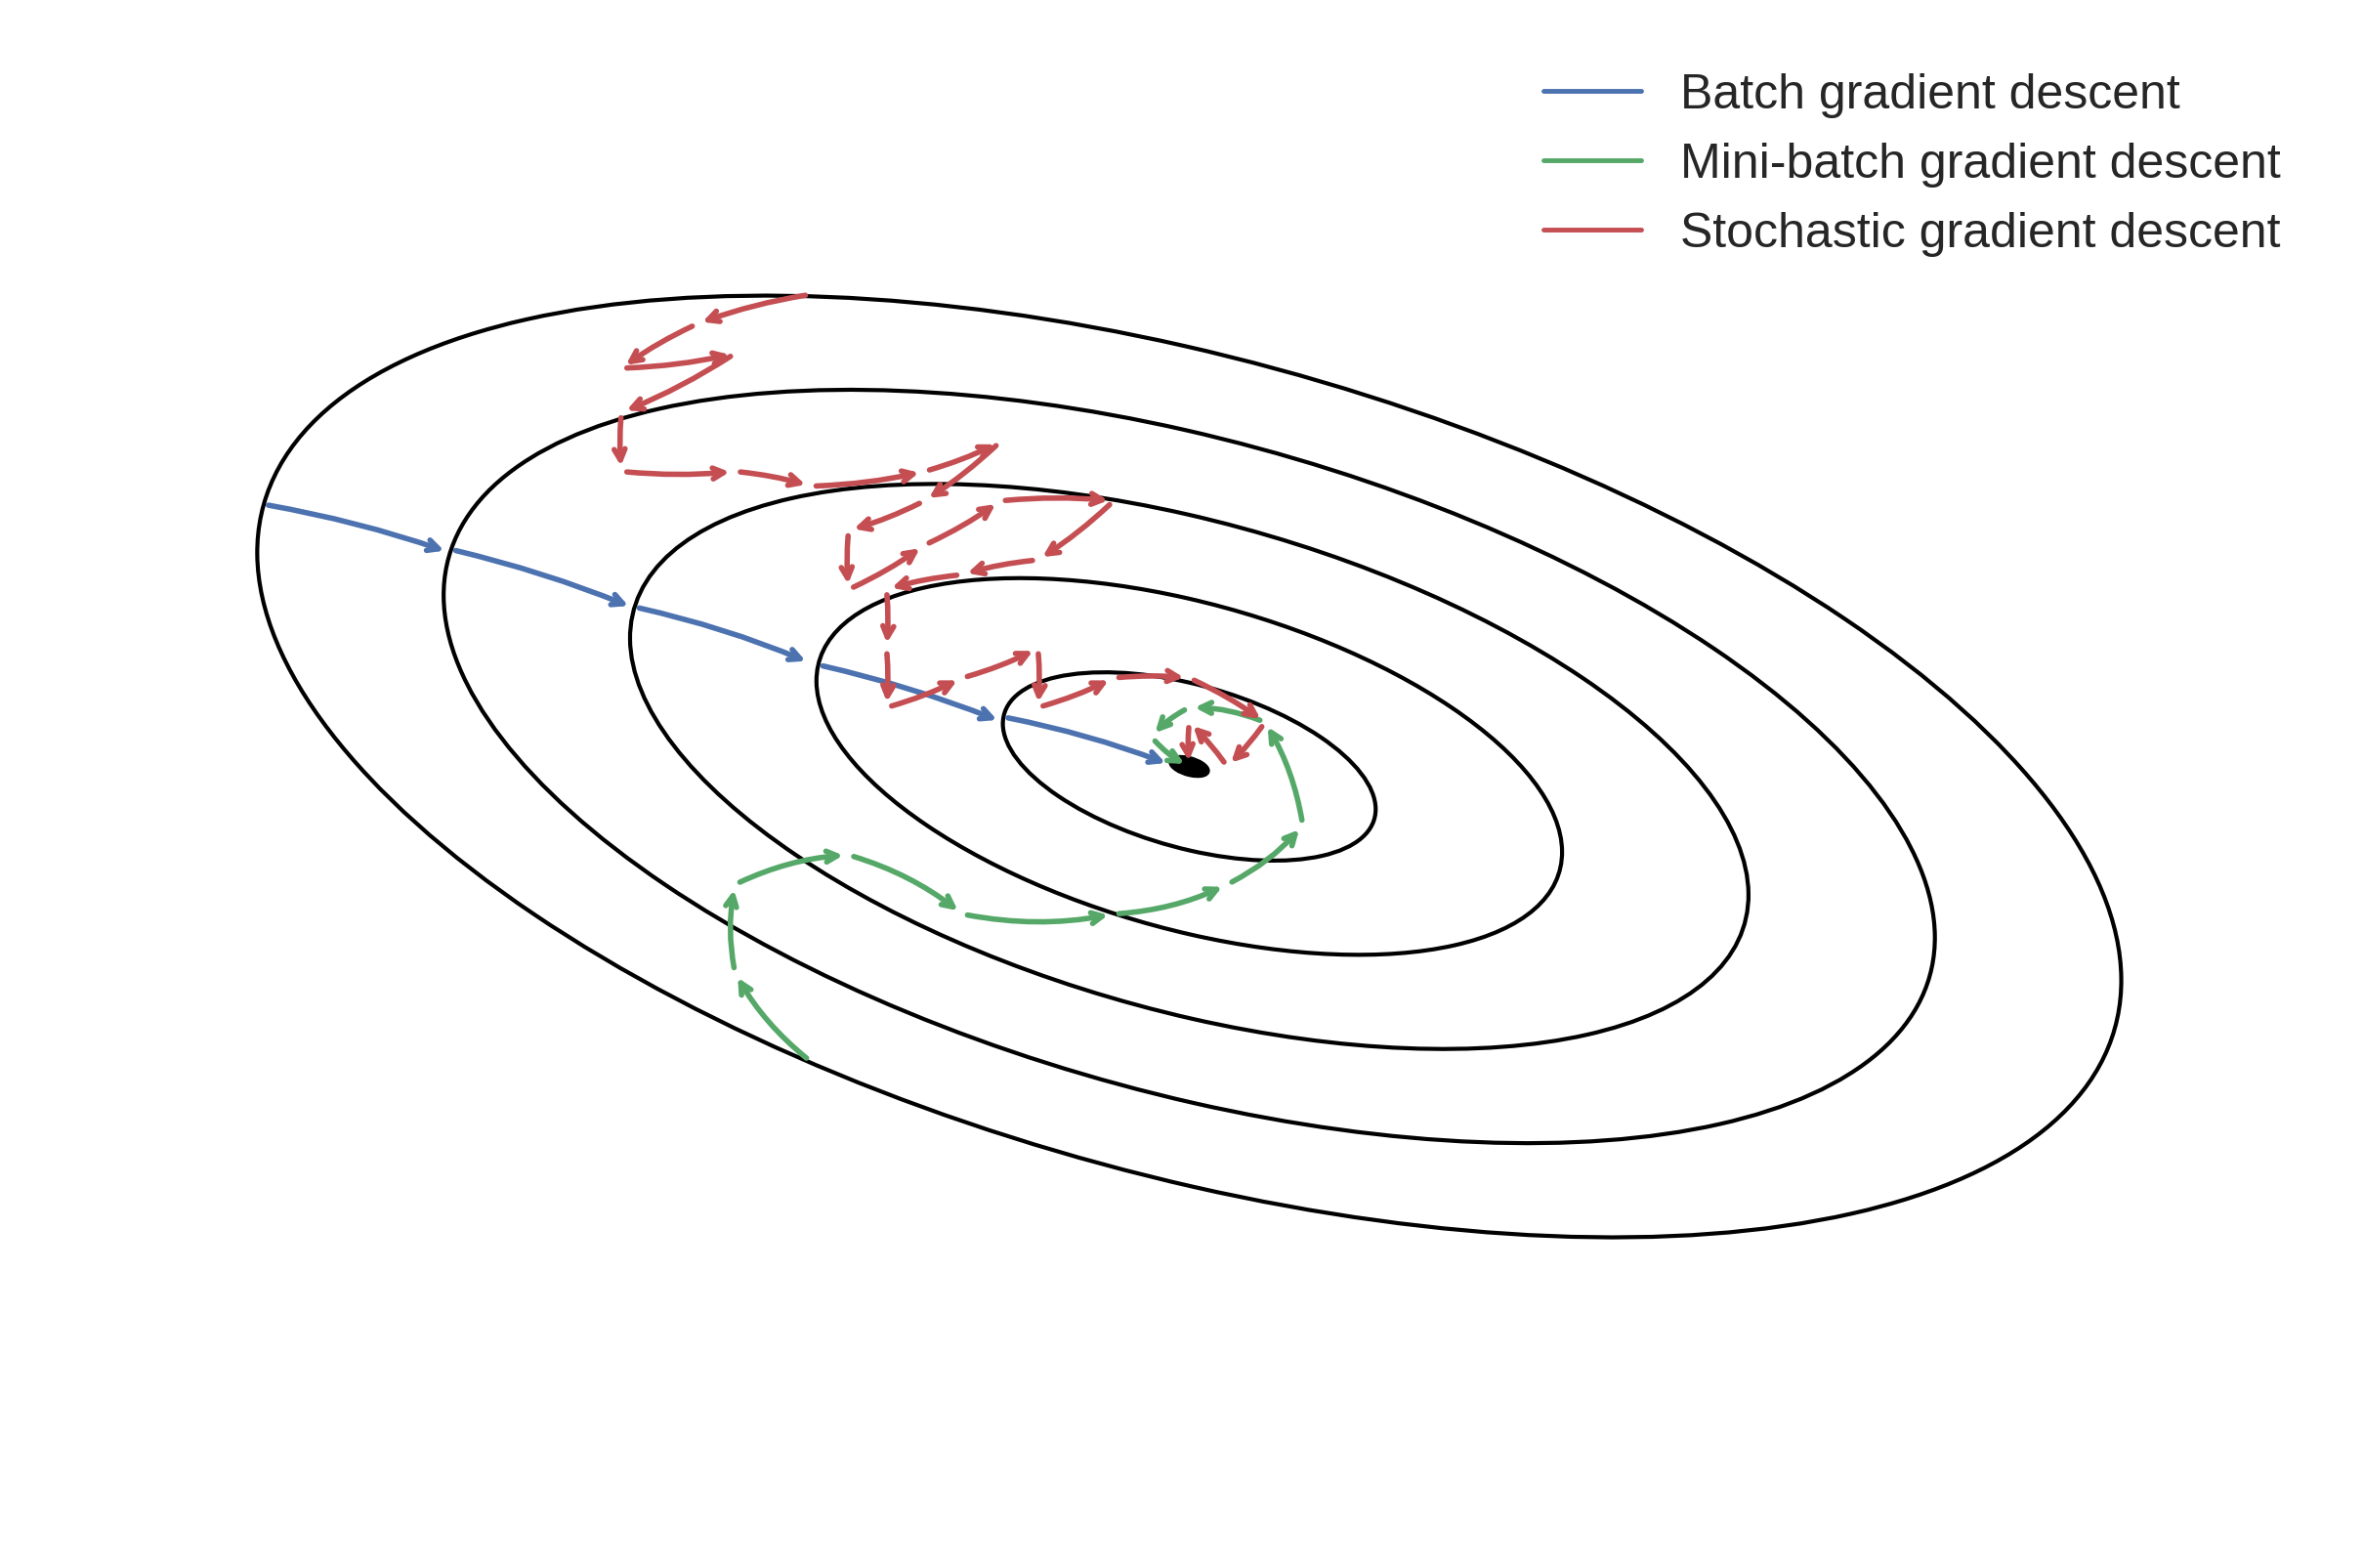
\includegraphics[width=\columnwidth]{gradient-descent_v2}%
	\end{figure}
	
	\subsection{Mini-Batch}
	
	As often in life the best solution is in the moderate mean rather than in extremism: \emph{Mini-Batch} is a powerful combination of \emph{Stochastic Gradient Descent (SDG)} and the \emph{Batch Gradient Descent}. By choosing common batch sizes like $64$, $128$, $256$ or $512$ it offers even for big training sizes ($m > 2,000$) huge performance improvements, because it can be computed in one GPU-clock without using only parts of the GPU stucking in organization overheads and it makes progress without processing the entire training set:\\
	
	Given: Split of dataset in batches of sizes greater than one: $(x^{\{t\}},y^{\{t\}})$
	\begin{lstlisting}[frame=single,caption={Mini-Batch Gradient Descent Algorithm}]
$shuffle([{\cal X}, {\cal Y}])$
for t in range(1,$\color{blue}batch\_size$):
   forward_prop(Input ${\cal X}^{\{t\}}$,
      Weight ${\cal W}^{[l]}$, Bias $b^{[l]}$)
   Costs ${\cal J}$ $\gets$ $\frac{1}{\color{blue}batch\_size} \times$
      $\sum_{i=1}^{\color{blue}batch\_size} {\cal L}oss(\hat{y^{\{t\}}},y^{\{t\})})$
   back_prop(${\cal A}^{[L]\{t\}} = \hat{y^{\{t\}}}$, $y^{\{t\}}$)
   ${\cal W}^{[l]} \gets {\cal W}^{[l]} - \alpha\times d{\cal W}^{[l]}$
   $b^{[l]} \gets b^{[l]} - \alpha\times db^{[l]}$
	\end{lstlisting}
	
	\begin{figure}
		\caption{Comparison of the Gradient Descent family performance on CIFAR-10}
		\resizebox {\columnwidth} {!} {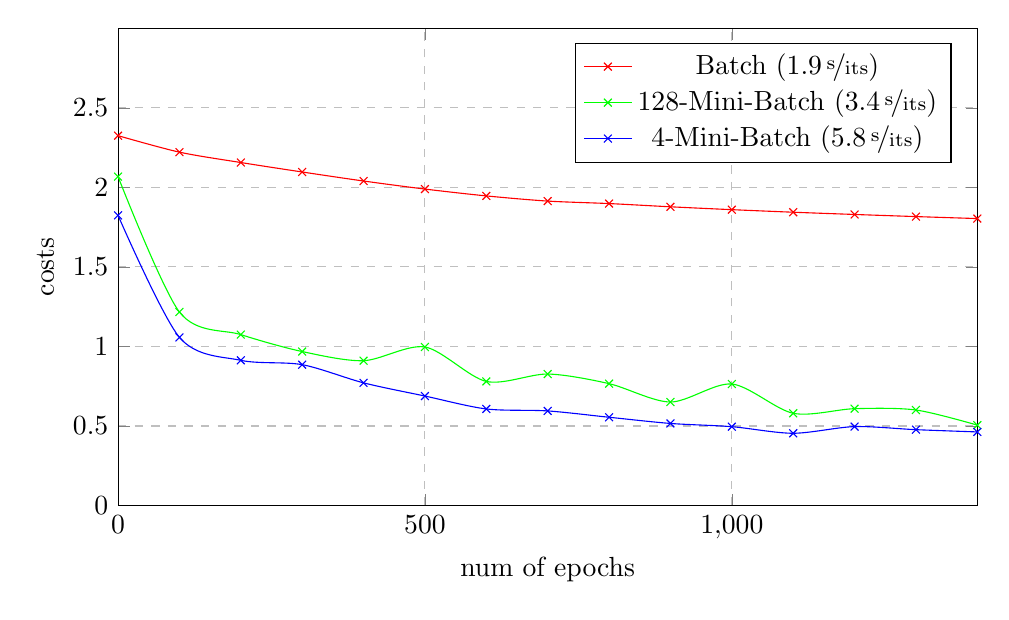
\begin{tikzpicture}
			\begin{axis}[
			xlabel={num of epochs},
			ylabel={costs},
			xmin=0, xmax=1400,
			ymin=0, ymax=3,
			scaled x ticks=false,
			smooth,
			xtick={0,500,1000},
			ytick={0,0.5,1,1.5,2,2.5},
			legend pos=north east,
			xmajorgrids=true,
			ymajorgrids=true,
			scale only axis=true,
			width=0.9\textwidth,
			height=0.5\textwidth,
			grid style=dashed,
			]
			
			\addplot[
			color=red,
			mark=x,
			]
			coordinates {%time per 1 Its: 1.89; train: 36,4%; test: 36,3%, alpha=0.009
				(0, 2.3248)(100, 2.2212)(200, 2.1560)(300, 2.0965)(400, 2.0398)(500, 1.9892)(600, 1.9462)(700, 1.9137)(800, 1.8981)(900, 1.8778)
				(1000, 1.8598)(1100, 1.8437)(1200, 1.8296)(1300, 1.8163)(1400, 1.8038)
			};
			
			\addplot[
			color=green,
			mark=x,
			]
			coordinates {%time per 1 Its: 3.36; train: 80,1%; test: 44,3%, alpha=0.009
				(0, 2.0675)(100, 1.2166)(200, 1.0746)(300, 0.9681)(400, 0.9106)(500, 0.9968)(600, 0.7803)(700, 0.8268)(800, 0.7664)(900, 0.6510)
				(1000, 0.7641)(1100, 0.5802)(1200, 0.6091)(1300, 0.6008)(1400, 0.5057)
			};
			
			\addplot[
			color=blue,
			mark=x,
			]
			coordinates {%time per 1 Its: 5.80; alpha=0.009
				(0, 1.8239)(100, 1.0573)(200, 0.9130)(300, 0.8857)(400, 0.7714)(500, 0.6885)(600, 0.6074)(700, 0.5950)(800, 0.5552)(900, 0.5163)
				(1000, 0.4959)(1100, 0.4546)(1200, 0.4965)(1300, 0.4772)(1400, 0.4630)
			};
			
			\legend{Batch (1.9\,\nicefrac{s}{its}), 128-Mini-Batch (3.4\,\nicefrac{s}{its}), 4-Mini-Batch (5.8\,\nicefrac{s}{its})}
			\end{axis}
			\end{tikzpicture}}
	\end{figure}
	
	\emph{Mini-Batch Gradient Descents} is able to improve our test accuracy by $22$\,\% only by giving the opportunity to reach a lower costs while using the same number of Epochs ($1,500$) despite the increasing duration per Epoch, whereas nearly \emph{Stochastic GD} is able to decrease the costs even faster, but it takes in my example with the \emph{CIFAR-10} dataset almost twice as long as \emph{Mini-Batch}, so it's not recommended.
	
	%%%%%%%%%%%%%%%%%%%%%%%%%%%%%%%%%%%%%%%%%%%%%%%%%%%%%%%%%%%
	
	\subsection{Momentum}
	
	According to Rumelhart, Hinton and Williams' paper on backpropagation learning~\cite{momentum}, \emph{Stochastic gradient descent with momentum} remembers the update $\Delta {\cal W}$ at each iteration and determines the next update as a linear combination of the current gradient and the previous update:
	
	\begin{align*}
	\Delta {\cal W} & \gets \beta \Delta {\cal W} - \alpha \nabla \cal{L}(W) \\
	{\cal W}        & \gets {\cal W} + \Delta {\cal W}
	\end{align*}
	
	\subsubsection{Running Average}
	
	Before presenting a concrete example of the most popular linear combination used for \emph{momentum} in deep learning, I first would like to start with a more basic idea of running average, the so called \emph{Simple moving average}:
	
	\begin{align*}
	SMA^{(n)}_{t-\tau} & = \frac{1}{n} \sum_{i=t-n}^{t}{\cal X}_{i}        \\
	n                  & \,\widehat{=}\,\text{memory}                      \\
	\tau               & \,\widehat{=}\,\text{group delay} = \frac{n-1}{2}
	\end{align*}
	
	Just summing over the last $n$ examples divided by $n$ (arithmetic mean) is for most cases a good idea, but the main disadvantage is, that it needs a memory (size: $n$) to fulfilled before using this technique is possible and it has got a delay about $\tau$. In cases, where the future is known and you want to draw something like a trend curve, you can shift the curve by $\tau$. Since Gradient Descent is a causal system, this is not an option.\\
	
	The \emph{Exponential moving average} in contrast is able to handle those problems. Towards \emph{bias correction} it has got even the ability to produce a great estimate even before the mean of $\approx \frac{1}{1-\beta}$ values is reached. With a weight of $\beta$, the current value will be added to the running average and afterward normalized for $\beta$, so that every value in the past of loses more and more influence as easily seen in the non-recursive formula: $\lim\limits_{i \rightarrow \infty}\beta^i = 0$.\\
	
	Biased moment estimate $EMA_{t}$:
	\begin{align*}
	EMA_{t} & = \beta\times EMA_{t-1} + (1-\beta)\times {\cal X}_{t}                          \\
	EMA_{t} & = \sum_{i=0}^{t} \beta^i(1-\beta) {\cal X}_{t-i} \Leftarrow\text{non-recursive}
	\end{align*}\\
	
	bias-corrected moment estimate $\widehat{EMA}_{t}$:
	\begin{align*}
	\widehat{EMA}_{t} & = \frac{EMA_{t}}{1-\beta^{t}}    \\
	\beta             & \,\widehat{=}\,\text{decay rate}
	\end{align*}
	
	\begin{figure}
		\caption{Illustration of both running averages on \emph{Dow-Jones} share prices}
		\resizebox {\columnwidth} {!} {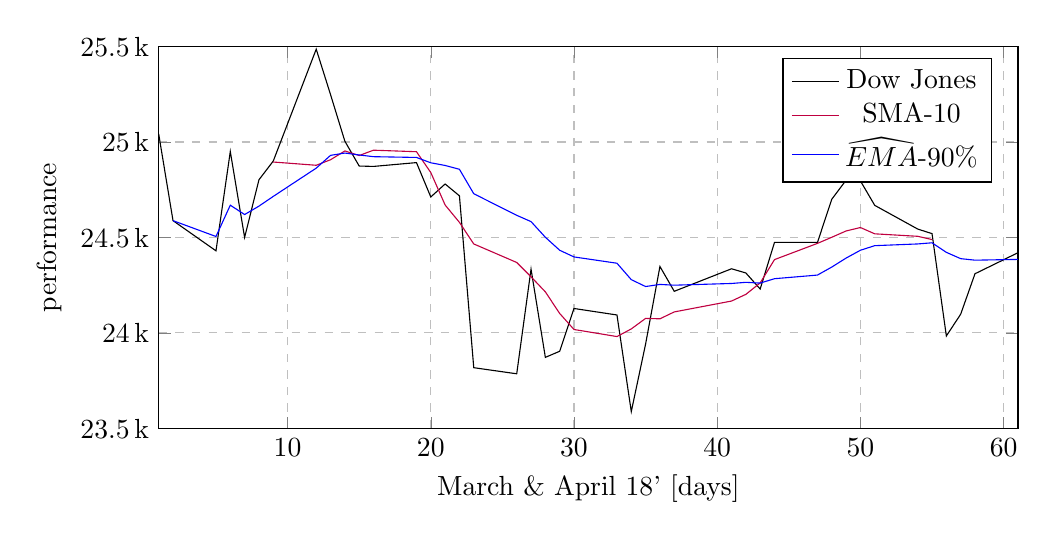
\begin{tikzpicture}
			\begin{axis}[
			xlabel={March \& April 18' [days]},
			ylabel={performance},
			xmin=1, xmax=61,
			ymin=23500, ymax=25500,
			scaled x ticks=false,
			legend pos=north east,
			scaled y ticks=base 10:-3,
			ytick scale label code/.code={},
			yticklabel={\pgfmathprintnumber{\tick}\,k},
			xmajorgrids=true,
			ymajorgrids=true,
			scale only axis=true,
			width=0.9\textwidth,
			height=0.4\textwidth,
			grid style=dashed,
			]
			
			\addplot[
			color=black,
			]
			coordinates {
				(1, 25042)(2, 24588)(5, 24430)(6, 24950)(7, 24500)(8, 24802)(9, 24900)
				(12, 25486)(13, 25248)(14, 25004)(15, 24874)(16, 24872)(19, 24892)
				(20, 24712)(21, 24780)(22, 24718)(23, 23818)(26, 23786)(27, 24334)(28, 23872)(29, 23904)
				(30, 24128)(33, 24094)(34, 23588)(35, 23942)(36, 24348)(37, 24218)
				(41, 24336)(42, 24314)(43, 24230)(44, 24474)(47, 24474)(48, 24700)(49, 24800)
				(50, 24796)(51, 24668)(54, 24544)(55, 24520)(56, 23984)(57, 24098)(58, 24310)(61, 24420)
			};
			
			\addplot[
			color=purple,
			]
			coordinates {
				(9, 24895)
				(12, 24878)(13, 24907)(14, 24953)(15, 24929)(16, 24957)(19, 24949)
				(20, 24840)(21, 24670)(22, 24579)(23, 24466)(26, 24369)(27, 24294)(28, 24215)(29, 24102)
				(30, 24018)(33, 23981)(34, 24021)(35, 24076)(36, 24074)(37, 24110)
				(41, 24167)(42, 24202)(43, 24262)(44, 24384)(47, 24469)(48, 24501)(49, 24534)
				(50, 24552)(51, 24519)(54, 24506)(55, 24489)
			};
			
			\addplot[
			color=blue,
			]
			coordinates {
				(2, 24588)(5, 24505)(6, 24669)(7, 24620)(8, 24664)(9, 24715)
				(12, 24863)(13, 24930)(14, 24942)(15, 24932)(16, 24923)(19, 24919)
				(20, 24891)(21, 24877)(22, 24857)(23, 24729)(26, 24616)(27, 24583)(28, 24501)(29, 24433)
				(30, 24398)(33, 24365)(34, 24279)(35, 24243)(36, 24254)(37, 24250)
				(41, 24259)(42, 24265)(43, 24261)(44, 24284)(47, 24303)(48, 24345)(49, 24392)
				(50, 24433)(51, 24457)(54, 24466)(55, 24472)(56, 24422)(57, 24389)(58, 24381)(61, 24385)
			};
			
			\legend{Dow Jones, SMA-10, $\widehat{EMA}$-90\%}
			\end{axis}
			\end{tikzpicture}}
	\end{figure}
	
	\subsubsection{Stochastic Gradient Descent with Momentum}
	
	Satisfying the requirements of a \emph{momentum} algorithm, in  \emph{exponential weighted average} old values loses more and more of significance because with every step the \emph{decay rate} as a factor of each gradient in each example gets minimized during to the increasing exponent (see non-recursive formula). These are leading factors for the acceptance of \emph{Exponential moving average} as the algorithm behind \emph{momentum}. To be detailed \emph{bias correction} is not part of the so-called \emph{Stochastic gradient descent with momentum}, because it's only relevant in the early learning period and makes computation more inefficient.
	\begin{lstlisting}[frame=single,caption={\texttt{Stochastic Gradient Descent with Momentum} Algorithm},label={lst:SGD_M}]
$\color{blue}\upsilon_{0} \gets \vv{0}$
for t in range(1,batch_size):
   forward_prop(Input $x^{\{t\}}$,
      Weight $W^{[l]}$, Bias $b^{[l]}$)
   Costs $J$ $\gets$ $\frac{1}{batch\_size} \times$
      $\sum_{i=1}^{batch\_size}Loss(\hat{y^{\{t\}}},y^{\{t\})})$
   back_prop($A^{[L]\{t\}} = \hat{y^{\{t\}}}$, $y^{\{t\}}$)
   $\color{blue}\upsilon_{dW} \gets \beta_1\times \upsilon_{dW} + (1-\beta_1)\times dW$
   $\color{blue}\upsilon_{db} \gets \beta_1\times \upsilon_{db} + (1-\beta_1)\times db$
   $W^{[l]} \gets W^{[l]} - \alpha\times \color{blue}\upsilon_{dW}$
   $b^{[l]} \gets b^{[l]} - \alpha\times \color{blue}\upsilon_{db}$
	\end{lstlisting}
	
	The main difference between \emph{Stochastic Gradient Descent without Momentum} can be seen in the algorithm in \autoref{lst:SGD_M}, using the results of our average system as gradients. With $\beta$ we introduce a new hyperparameter in order to efficiently update new incoming values called exponential decay rate for moment estimate. According to the paper owners, a value round about $0.9$ seems useful, so there is the potential, but not the actual need to tune this hyperparameter, because tuning the learning rate or the regularization factor takes better improvements to the model.
	
	\subsection{RMSProp}
	
	The principle of \emph{RMSProp}~\cite{rmsprop} is in most terms the same as it of \emph{Gradient Descent with Momentum} besides the fact, that instead of computing exponential running average without any scale, a squared version of the input into the average modulation is useful, because a massive increase in $db$ (and $\varsigma$) get caught by the final gradient $\nicefrac{db}{\sqrt{\varsigma}}$ (also illustrated in \autoref{fig:RMSProp}). Whenever you will, unfortunately, do an extraordinary high step going into the wrong direction e\,g. in oscillation, our running average $\varsigma$ will also increase significantly (because of the square). Due to the fact, that our final gradient is the fraction of the current gradient divided by the square root of the running average $\varsigma$, the wrong and high value gets divided by a higher running average in order to get fixed in a more stable range.\\
	
	\begin{figure}
		\caption{Non-optimized learning algorithms often suffer of a high oscillation in $b$ or other dimensions whereas Momentum seems to be more resistant}
		\label{fig:RMSProp}
		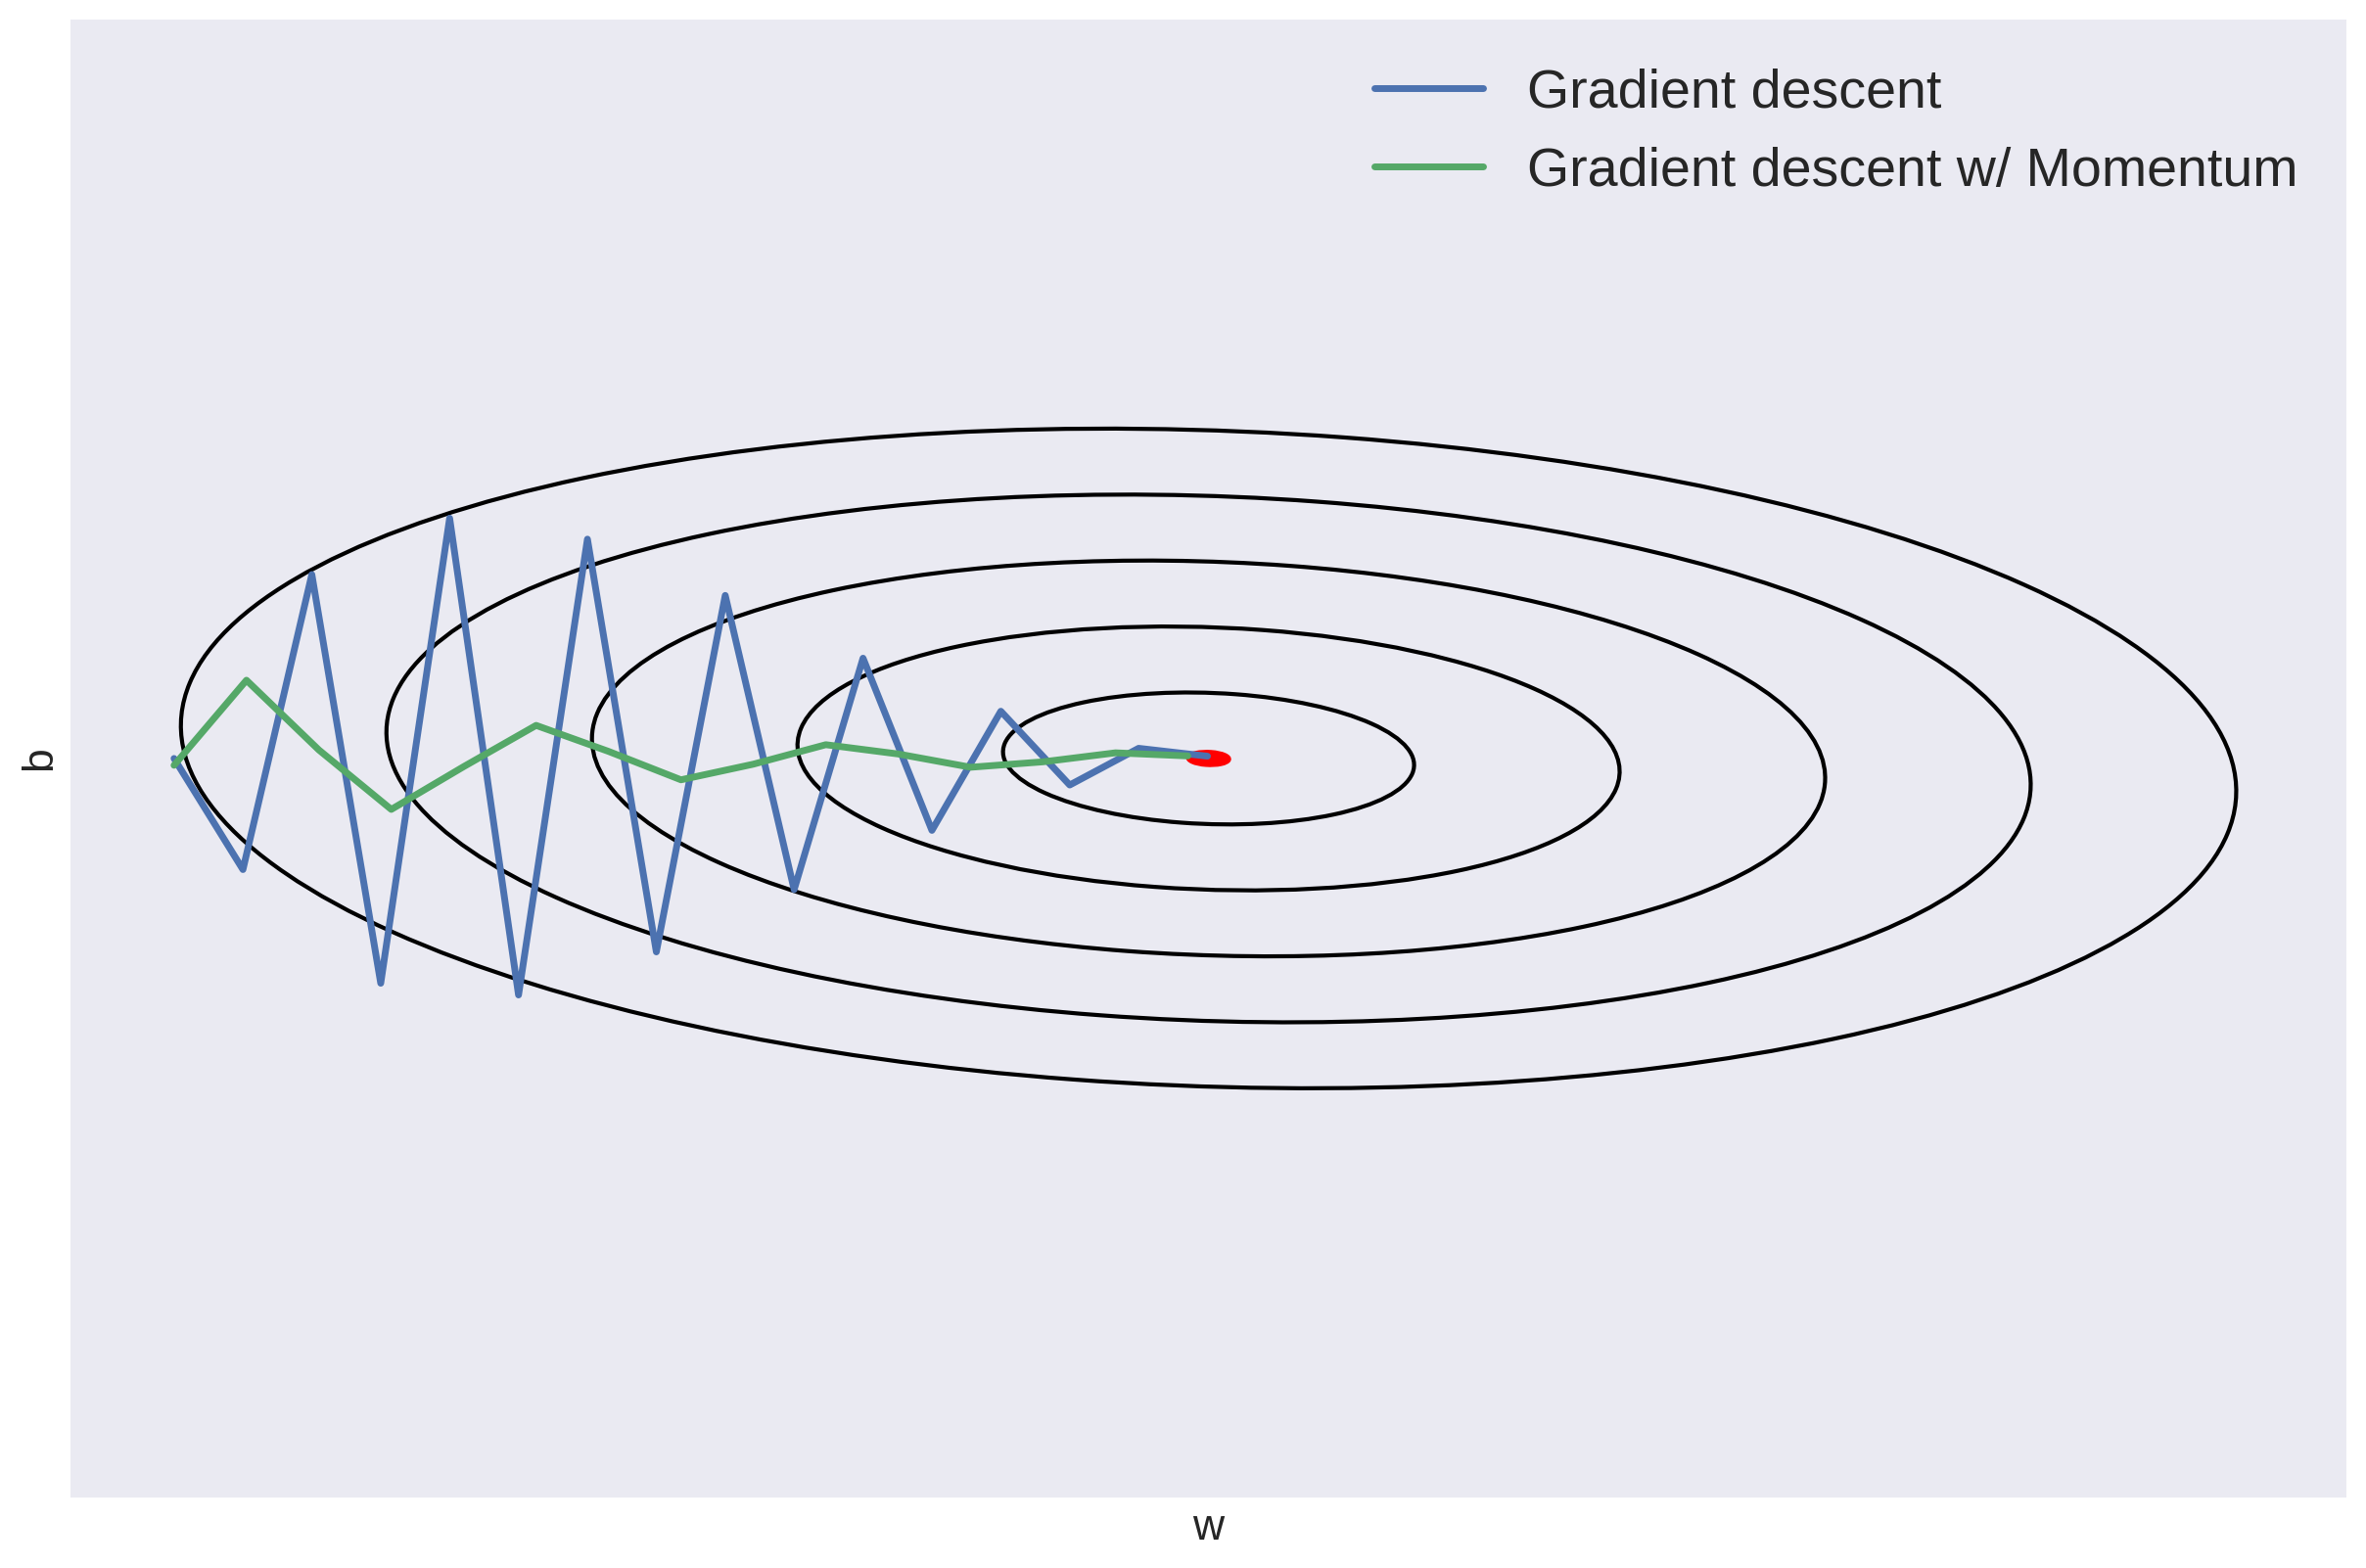
\includegraphics[width=\columnwidth]{momentum_v2}%
	\end{figure}
	
	E.\,g. if we consider, that our running average for $db$ has a full memory and currently stays on $\varsigma = 2$, because all our previous gradients are in a normal behavior (final and somehow fixed gradient: $\nicefrac{1.42}{\sqrt{2}} = 1$). Suddenly our gradient $db$ jumps up to $6$, so our new running average denotes by using a $\beta_2$ of $0.9$ to $\varsigma = 0.9\times2 + 0.1\times36 = 5.4$, but luckily our final gradient doesn't change that much: $\nicefrac{6}{\sqrt{5.4}} \approx 2.58$.\\
	
	In the previously simple example, we changed our final gradient by round about half the original value. This would be a too big impact on the final learning algorithm since it should only behave as assistance system preventing \emph{exploiting gradients} and not as a normalizing system. The plant archive this balance by choosing a very low hyperparameter $\beta_2 = 0.999$ having as same as in \emph{Momentum} no need of real tuning.
	
	N.\,B. the "hyperparameter`` $\epsilon$ can also be tuned because formally it is actually a hyperparameter, but since its only purpose is to grantee numerical stability in the denominator, there is no actual sense to handle it like this.\\\\
	
	
	\begin{lstlisting}[frame=single,caption={\texttt{Stochastic Gradient Descent with RMSProp} Algorithm}]
$\color{blue}\varsigma_0 \gets \vv{0}$
$\color{blue}\epsilon \approx 10^{-8}$
for t in range(1,batch_size):
   forward_prop(Input ${\cal X}^{\{t\}}$,
      Weight ${\cal W}^{[l]}$, Bias $b^{[l]}$)
   Costs ${\cal J}$ $\gets$ $\frac{1}{batch\_size} \times$
      $\sum_{i=1}^{batch\_size} {\cal L}oss(\hat{y^{\{t\}}},y^{\{t\})})$
   back_prop(${\cal A}^{[L]\{t\}} = \hat{y^{\{t\}}}$, $y^{\{t\}}$)
   $\color{blue}\varsigma_{d{\cal W}} \gets \beta_2\times \varsigma_{d{\cal W}} + (1-\beta_2)\times d{\cal W}^2$
   $\color{blue}\varsigma_{db} \gets \beta_2\times \varsigma_{db} + (1-\beta_2)\times db^2$
   ${\cal W}^{[l]} \gets {\cal W}^{[l]} - \alpha\times \color{blue}\frac{d{\cal W}}{\sqrt{\varsigma_{d{\cal W}}}+\epsilon}$
   $b^{[l]} \gets b^{[l]} - \alpha\times \color{blue}\frac{db}{\sqrt{\varsigma_{db}}+\epsilon}$
	\end{lstlisting}
	
	\subsection{ADAM}
	
	All those optimizers have got in mind, that they offer the ability for more stable and faster learning. But in order to archive this goal, a simple implementation of the current state-of-the-art optimizer \emph{ADAM} isn't enough, when not looking at the same time on your behind: The learning rate $\alpha$ can e.\,g. also highly increased and other hyper-parameters have to tuned another time.
	
	The tuning process of hyper-parameters is a progress you have to think about for a moment. First, you need to be aware of all relevant and tunable hyper-parameters and its ranges ignoring such unimportant ones like $\epsilon$, $\beta_1$ or $\beta_2$, to be more focused on the real advantages. A good way to start is with optimizing the learning rate $\alpha$, the mini-batch-size and the number of hidden units; The number of layers and the learning rate decay hyper-parameter takes also some improvements. Secondly, you either sample these five hyper-parameters in a grid by choosing 10 values each, or you choose e.\,g. 50 random values and afterward you will zoom into the region of the lowest cost after some iteration of the development set and start sampling again in this small region. Ordering the different values for the hyper-parameters in a grid has the main disadvantage, that you only try for every parameter a small non-distinct number of values: By training the learning rate $\alpha$ and $\epsilon$ for numerical stability in a grid 5 values each e.\,g. you will ignore the fact that $\alpha$ is more important than $\epsilon$ and only 5 redundant values of $\alpha$ is trained in contrast to 25 distinct values using randomized sampling.
	
	Transforming the scale of each hyperparameter to a logarithmically scale is also in most cases a good idea because, by this technique, you can shuffle your concrete values efficiently e.\,g. between $0.0001$ and $1$ for $\alpha$ or between $0.9$ and $0.999$ for $\beta_1$ in exponential weighted average in \emph{Momentum}.
	
	\begin{lstlisting}[frame=single,caption={\texttt{Stochastic Gradient Descent with ADAM} Algorithm},label={lst:ADAM}]
for t in range(1,batch_size):
   forward_prop(Input ${\cal X}^{\{t\}}$,
      Weight ${\cal W}^{[l]}$, Bias $b^{[l]}$)
   Costs ${\cal J}$ $\gets$ $\frac{1}{batch\_size} \times$
      $\sum_{i=1}^{batch\_size} {\cal L}oss(\hat{y^{\{t\}}},y^{\{t\})})$
   back_prop(${\cal A}^{[L]\{t\}} = \hat{y^{\{t\}}}$, $y^{\{t\}}$)
      $\color{ForestGreen}Momentum:$
   $\upsilon_{d{\cal W}} \gets \beta_1\times \upsilon_{d{\cal W}} + (1-\beta_1)\times d{\cal W}$
   $\upsilon_{db} \gets \beta_1\times \upsilon_{db} + (1-\beta_1)\times db$
      $\color{ForestGreen}RMSProp:$
   $\varsigma_{d{\cal W}} \gets \beta_2\times \varsigma_{d{\cal W}} + (1-\beta_2)\times d{\cal W}^2$
   $\varsigma_{db} \gets \beta_2\times \varsigma_{db} + (1-\beta_2)\times db^2$
      $\color{ForestGreen}Bias\,correction:$
   $\color{blue}[\widehat{\upsilon_{d{\cal W}}}, \widehat{\upsilon_{db}}] \gets \frac{[\upsilon_{d{\cal W}}, \upsilon_{db}]}{1 - \beta_1^{its}}$
   $\color{blue}[\widehat{\varsigma_{d{\cal W}}}, \widehat{\varsigma_{db}}] \gets \frac{[\varsigma_{d{\cal W}}, \varsigma_{db}]}{1 - \beta_2^{its}}$
      $\color{ForestGreen}Gradient\,update:$
   ${\cal W}^{[l]} \gets {\cal W}^{[l]} - \alpha\times \frac{\color{blue}\widehat{\upsilon_{d{\cal W}}}}{\sqrt{\color{blue}\widehat{\varsigma_{d{\cal W}}}}+\epsilon}$
   $b^{[l]} \gets b^{[l]} - \alpha\times \frac{\color{blue}\widehat{\upsilon_{db}}}{\sqrt{\color{blue}\widehat{\varsigma_{db}}}+\epsilon}$
	\end{lstlisting}
	
	\emph{ADAM} derived from \emph{adaptive moment estimation} is the fastest and most intelligent state-of-the-art optimizing algorithm introduced by Kingma and Ba~\cite{adam} combining \emph{Momentum}, \emph{RMSProp} and \emph{Bias correction} with $\beta_1 = 0.9$ and $\beta_2 = 0.999$ (see algorithm in \autoref{lst:ADAM}).
	
	\begin{figure}
		\caption{Comparison of learning algorithms according to~\cite{adam}}
		\includegraphics[width=\columnwidth]{ADAM}%
		%according to original paper
	\end{figure}
	
	\begin{figure}
		\caption{CIFAR-10 optimizer comparison}
		\resizebox {\columnwidth} {!} {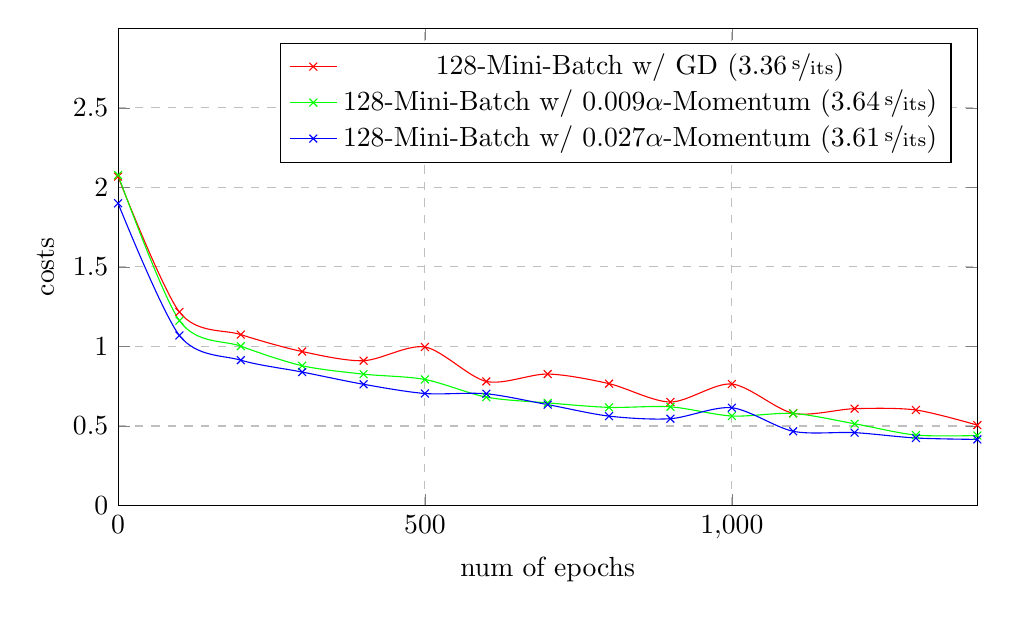
\begin{tikzpicture}
			\begin{axis}[
			xlabel={num of epochs},
			ylabel={costs},
			xmin=0, xmax=1400,
			ymin=0, ymax=3,
			scaled x ticks=false,
			smooth,
			xtick={0,500,1000},
			ytick={0,0.5,1,1.5,2,2.5},
			legend pos=north east,
			xmajorgrids=true,
			ymajorgrids=true,
			scale only axis=true,
			width=0.9\textwidth,
			height=0.5\textwidth,
			grid style=dashed,
			]
			
			\addplot[
			color=red,
			mark=x,
			]
			coordinates {%time per 1 Its: 3.36; train: 80,1%; test: 44,3%, alpha=0.009
				(0, 2.0675)(100, 1.2166)(200, 1.0746)(300, 0.9681)(400, 0.9106)(500, 0.9968)(600, 0.7803)(700, 0.8268)(800, 0.7664)(900, 0.6510)
				(1000, 0.7641)(1100, 0.5802)(1200, 0.6091)(1300, 0.6008)(1400, 0.5057)
			};
			
			\addplot[
			color=green,
			mark=x,
			]
			coordinates {%time per 1 Its: 3.64; train: 84,9%; test: 43,6%, alpha=0.009, beta=0.9
				(0   , 2.0773)(100 , 1.1624)(200 , 1.0019)(300 , 0.8790)(400 , 0.8261)(500 , 0.7927)(600 , 0.6817)(700 , 0.6456)(800 , 0.6173)(900 , 0.6208)
				(1000, 0.5630)(1100, 0.5791)(1200, 0.5144)(1300, 0.4432)(1400, 0.4405)
			};
			
			\addplot[
			color=blue,
			mark=x,
			]
			coordinates {%time per 1 Its: 3.61; train: 85,1%; test: 43,0%, alpha=0.027, beta=0.9
				(0, 1.9000)(100, 1.0691)(200, 0.9138)(300, 0.8394)(400, 0.7624)(500, 0.7045)(600, 0.7027)(700, 0.6346)(800, 0.5623)(900, 0.5461)
				(1000, 0.6149)(1100, 0.4669)(1200, 0.4586)(1300, 0.4248)(1400, 0.4160)
			};
			
			\legend{128-Mini-Batch w/ GD (3.36\,\nicefrac{s}{its}), 128-Mini-Batch w/ 0.009$\alpha$-Momentum (3.64\,\nicefrac{s}{its}), 128-Mini-Batch w/ 0.027$\alpha$-Momentum (3.61\,\nicefrac{s}{its})}
			\end{axis}
			\end{tikzpicture}}
	\end{figure}
	
	\subsection{Final Chapter-Remark}
	
	Concluding with one of the most complex and even most relevant topic when talking about Optimization Techniques in deep neural networks, you should note, that even if nowadays \emph{ADAM} is the best choice, in maybe 5 years it'll be totally outdated choosing \emph{ADAM}. There will be better algorithms which save e.\,g. another minute in one hour and you'll be naive if you won't use them. Maybe you are even struggling with implementing \emph{ADAM} on your own, but that's okay. You don't have to implement this error-like algorithm on your own, you should only know how modern optimization techniques safes times, so you confide \emph{ADAM} or how the latest algorithm will be called and don't notice them as a mysterious black box.\\
	As a black box, you also won't longer observe \emph{Batch Normalization} due to the next chapter.
	
	%%%%%%%%%%%%%%%%%%%%%%%%%%%%%%%%%%%%%%%%%%%%%%%%%%%%%%%%%%%%%%%%%%%%%%%%%%%%%%%%%%%%
	
	\section{Batch Normalization}
	
	According to S.~Ioffe and C.~Szegedy~\cite{batchnorm} training a neural network is complicated, because of \emph{Internal Covariance Shift}: The inputs to each layer are affected by the parameters of all preceding layers, so that continuously adapting to different distributions instead of real learning is necessary. Furthermore, there is the problem, that small changes to early network weights amplify as it becomes deeper. One well-known technique is to normalize the input data $\cal X$, but why not only normalize the global input and normalize the input to every layer $\cal Z$? This is exactly what Batch Norm is about.
	
	Additionally, it introduces a slight regularization when using Mini-Batches by adding noise of different mean and variance each mini-batch (\emph{Stochastic Gradient Descent} is, in this case, useless because normalizing only one input data isn't possible).\\
	
	Taking a short look onto the activation function, we are able to observe, that it is useful to normalize before applying the activation function $tanh$. This lays down to the fact, that we implicit also fix the problem of vanishing gradients by keeping most weights in a range of $-1$ and $1$ (normal distributed: $\sigma = 1$, $\mu = 0$), which is in the $tanh$-function the area, where there are the highest possible gradients. Without Batch Norm, we can get stuck in very high or low gradients slowing down the learning process. Choosing another activation function like e.\,g. \emph{ReLU - rectified linear unit} $f(x) = x^+ = max(0,x)$ in the hidden layers and a \emph{softmax} (multi-class classification) or \emph{tanh} (single-class classification) for the output layer in order to make predictions between 0 and 1 establishing the probability of its occurrence might also one possible solution to the \emph{vanishing gradient} problem. But this doesn't fix the slow learning process caused by \emph{internal covariance shift} (see above).
	
	\begin{figure}
		\caption{$tanh$-function}
		\resizebox {\columnwidth} {!} {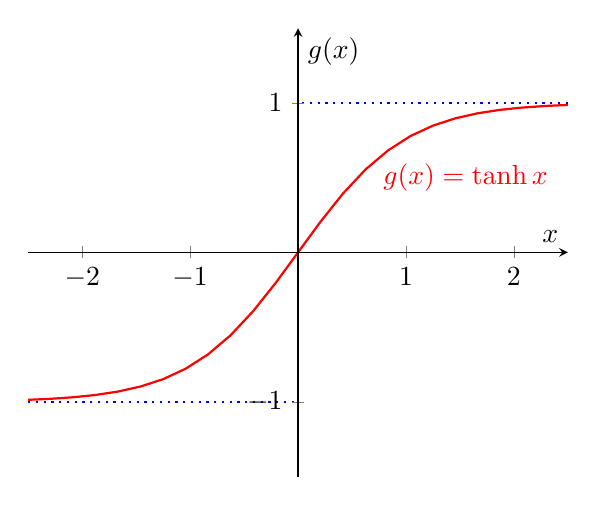
\begin{tikzpicture}
			\begin{axis}[
			xmin=-2.5, xmax=2.5,
			ymin=-1.5, ymax=1.5,
			axis lines=center,
			axis on top=true,
			domain=-2.5:2.5,
			ylabel=$g(x)$,
			xlabel=$x$,
			]
			
			\addplot [mark=none,draw=red, thick] {tanh(\x)};
			\node [right, red] at (axis cs: 0.7,0.5) {$g(x) = \tanh x$};
			
			%% Add the asymptotes
			\draw [blue, dotted, thick] (axis cs:-2.5,-1)-- (axis cs:0,-1);
			\draw [blue, dotted, thick] (axis cs:+2.5,+1)-- (axis cs:0,+1);
			\end{axis}
			\end{tikzpicture}}
	\end{figure}
	
	Before implementing BatchNorm $BN_{\gamma,\beta}(x_i)$ with $tanh$ or the outdated $sigmoid$-function you should be aware of the fact, that both are almost non-linear in the region between $-1$ and $1$, which would reduce the complexity significantly, if you not always shift and scale to $\sigma = 1$ and $\mu = 0$, but introduce two learnable parameters $\gamma$ and $\beta$ (not confuse with $\beta$ in \emph{Momentum}) deciding themselves which is the best scale and shift. If the neural network learns e.\,g. for some layer a $\gamma$ of  $\sqrt{\sigma^2 + \epsilon}$ and a $\beta$ of $\mu$ you can conclude that $y_i = x_i$ must hold and Batch Norm takes no effect.
	
	\begin{lstlisting}[frame=single,basicstyle=\linespread{1.5}\ttfamily,caption={\texttt{Batch-Norm} Algorithm}]
$\epsilon = 10^{-8}$
$\cal{B}$$ = \{x_{1\dots m}\}, m > 1$ $\color{ForestGreen}\Leftarrow Mini-Batch$
$\color{ForestGreen} \text{mini-batch mean:}$
$\mu_{\cal{B}} \gets \frac{1}{m}\sum_{i=1}^{m}x_i$
$\color{ForestGreen} \text{mini-batch variance:}$
$\sigma_{\cal{B}}^2 \gets \frac{1}{m}\sum_{i=1}^{m}(x_i - \mu_{\cal{B}})^2$
$\color{ForestGreen} \text{normalize:}$
$\hat{x_i} \gets \frac{x_i - \mu_{\cal{B}}}{\sqrt{\sigma_{\cal{B}}^2 + \epsilon}}$
$\color{ForestGreen} \text{scale and shift:}$
$y_i \gets {\color{blue}\gamma} \hat{x_i} + {\color{blue}\beta} \equiv BN_{\gamma,\beta}(x_i)$
	\end{lstlisting}
	
	\begin{lstlisting}[frame=single,basicstyle=\linespread{1.5}\ttfamily,caption={\texttt{Batch-Norm} Algorithm in a Neural-Net Layer}]
${\cal Z}^{[l]}  \gets {\cal W}^{[l]} a^{[l-1]} + \color{red}\cancelto{\vv{0}}{b^{[l]}}$
${\cal Z}^{[l]}_{norm} \gets \frac{{\cal Z}^{[l]} - \mu_{\cal{B}}}{\sqrt{\sigma_{\cal{B}}^2 + \epsilon}}$
$\hat{{\cal Z}^{[l]}} \gets \gamma^{[l]}{\cal Z}^{[l]}_{norm} + \beta^{[l]}$
	\end{lstlisting}
	
	N.\,B. that you don't even need the bias $b$ anymore (you can either remove it or replace it with the zero-vector $\vv{0}$), because you will shift the input by $\beta$ so it would be redundant to maintain the bias, too. Secondly, you can also decide to use in contrast to my algorithms in this chapter another learning function like \emph{ADAM}, but for simplicity, I decided to use \emph{Gradient Descent}.
	
	\begin{lstlisting}[frame=single,basicstyle=\linespread{1.5}\ttfamily,caption={\texttt{Batch-Norm} Algorithm in a Deep Neural-Network}]
for t in range(1,$batch\_size$):
   forward_prop(Input ${\cal X}^{\{t\}}$,
      Weight ${\cal W}^{[l]}$, $\color{red}\xcancel{\text{Bias} b^{[l]}}$)
   Costs ${\cal J}$ $\gets$ $\frac{1}{batch\_size} \times$
      $\sum_{i=1}^{batch\_size} {\cal L}oss(\hat{y^{\{t\}}},y^{\{t\})})$
   back_prop(${\cal A}^{[L]\{t\}} = \hat{y^{\{t\}}}$, $y^{\{t\}}$)
   ${\cal W}^{[l]} \gets {\cal W}^{[l]} - \alpha\times d{\cal W}^{[l]}$
   $b^{[l]} \gets b^{[l]} - \alpha\times db^{[l]}$
   $\color{blue}\beta^{[l]} \gets \beta^{[l]} - \alpha\times d\beta^{[l]}$
   $\color{blue}\gamma^{[l]} \gets \gamma^{[l]} - \alpha\times d\gamma^{[l]}$
	\end{lstlisting}
	
	\begin{figure}
		\caption{Distributions in the last hidden layer (15, 50, 85 percentiles)~\cite{batchnorm}}
		\includegraphics[width=\columnwidth]{BN}\\
	\end{figure}
	
	\subsection{Final Advices}
	
	The original paper had got space left for some advanced advises how to fit \emph{Batch Norm} best into your existing neural network. You have to keep that in mind, because just implementing \emph{Batch Normalization} without rethinking your hyperparameter won't be that successful:
	\begin{itemize}
		\item Increase learning rate (by factor \textasciitilde{}5 onwards), because Batch Norm adds more stability to the learning process only focused on the decision boundary itself in a more or less fixed distribution.
		\item Remove dropout since Batch Norm already included a slight regularization
		\item Reduce $L_2$ Weight-Regularization (by \textasciitilde{}5)
		\item Accelerate learning rate decay because convergence gets improved
		\item Shuffle training examples more thoroughly because Batch Norm relies for an optimal distribution-fix on real randomness with respect to each mini-batch. Each mini-batch should have approximately the same distribution as all data in order to have a fixed distribution.
	\end{itemize}
	
	As already mentioned in my final chapter-remark in the \emph{Optimizer}-section you can implement \emph{Batch Norm} on your own, but you have to adapt also your backpropagation algorithm and be aware of it on testing time. \emph{Gradient Checking} will be one of the rare techniques of verifying that you implement your backpropagation algorithm including Batch Norm correctly, but most of the time a little mistake in your program easily caused when dealing with such complex algorithms, can significantly disturb your model performance. So if you have an overall understanding Batch Normalization you are better staying at a pre-programmed AI-library as e.\,g. \emph{TensorFlow} instead of program everything on your own.
	
	%%%%%%%%%%%%%%%%%%%%%%%%%%%%%%%%%%%%%%%%%%%%%%%%%%%%%%%%
	
	\section{Feature-Optimization}
	
	Personally, I realized during my seminar work that this chapter is one of the important ones when dealing with Optimization in Deep Learning, not because it has got the biggest impact, but because it's an underestimated optimization technique. Jesse Moore claims:
	\blockquote{You should spend time developing tools to analyze, present, and study your input data. [\dots] Avoid thinking of data as merely an input. All data has hidden features that hold immense predictive power if you can extract them. \textbf{Data is greater than model design, and model design is greater than parameter optimization.}}
	
	And that's basically how it is: More important than disturbing the pipeline in the middle and forcing with any power you can obtain in order to get your result you want, machine learning is more about thinking and understanding your features. If you don't analyze what's really relevant for your prediction you get lost in spending computational power for heating your home and not more.
	
	Speaking from the perspective of the cartoon in \autoref{fig:cartoon}: Instead of improving how to stir your pile best, you're better with decrease your pile's height.
	
	\blockquote{With too little data, you won’t be able to make any conclusions that you trust. With loads of data you will find relationships that aren’t real [\dots] \textbf{Big data isn’t about bits, it’s about talent.} \\-- Douglas Merrill}
	
	\begin{figure}
		\begin{center}
			\caption{The real importance in Deep Learning \href{https://xkcd.com/1838/}{$@xkcd^{1838}$}}
			\label{fig:cartoon}
			\includegraphics[width=\columnwidth]{cartoon}
		\end{center}
	\end{figure}
	
	\subsection{Possible Feature Reductions}
	
	To get in touch with Feature Optimization we should first start asking ourselves what actual enhancements we can reach.
	
	E.\,g. let's assume our Logistic Regression Network of $\{3072, 10\}$ layer dimensions on the CIFAR-10 dataset using the approach that every RGB-value on every pixel in our image should be one feature being computational inefficient. But that's actually not the best representation and has got a lot of redundancy: Nearby pixels are highly dependent and even in the corners of the image or in the color there is no new information. Shannon's entropy states that there have to be a better representation as e.\,g. used in \emph{JPEG}-compression or grayscaling.
	
	\subsection{Grayscaling}
	
	Grayscaling is one example of a \textbf{input-independent technique}, because some brilliant scientists have observed a magic formula of how 3-channel-color images looks best for human eyes according to the fact that we are most sensitive for green color: $Y_{Gray} = 0.2126\times R_{ed} + 0.7152\times G_{reen} + 0.0722\times B_{lue}$. With this method, we also get a high contrast. This has got huge performance benefits because the computation complexity is linear, but on the other hand, we have the main disadvantage, that we first need to observe this static formula transforming the features. In most cases and even when handling with non-image data we haven't got that ability, even when keeping in mind that the sense of making predictions with a Deep Neural Network is to be not relevant on which detailed feature correlation you might have. If you start analyzing like this you should think twice if a Neural Net is what you really want.\\
	
	Let's consider we have got a colored image of \emph{Lena} the most famous playboy-girl in computer science. If we grayscale her we can reduce our feature size by 3: Now we have $\{262.144, 10\}$ instead of $\{786.432, 10\}$.
	\begin{figure}
		\caption{Lena in Color and Gray}
		\includegraphics[width=0.45\columnwidth]{lena}
		$\Rightarrow$
		\includegraphics[width=0.45\columnwidth]{lena_sw}
	\end{figure}
	\begin{figure}
		\caption{Lena's scatter plot in R-G-B-domain}
		\includegraphics[width=\columnwidth]{lena_scatter}
	\end{figure}
	
	\subsection{DCT / DFT}
	
	But there is another group of feature reduction techniques namely \textbf{input-dependent techniques}. Examples might be \emph{Discrete Cosine Transformation -- DCT} or \emph{Discrete Fourier Transformation -- DFT} being able to change an input's data to an abstract frequency representation, whereas low frequencies are that ones who gives the global structure towards an image and high frequencies are responsible for exact borders. Cutting high frequencies only has the disadvantage, that your image gets a little bit of fuzziness, but you don't lose that many information. This method is therefore state-of-the-art in image compression.
	
	\subsection{PCA}
	
	Another possible feature reduction technique is to use \emph{Principal Component Analysis} also called \emph{PCA}, which is state-of-the-art in Deep Learning. Conceptual it is completely the same as for \emph{DCT}, but we transform our data in the eigenvectors domain, where each eigenvector is orthonormal to all other eigenvectors scaled by his eigenvalue. So we project our features to those top-level eigenvectors, which have got the highest eigenvalues because in this dimension there is the highest variance and we lost almost no information. This algorithm is called \emph{principal axis theorem}.
	
	In \autoref{fig:PCA_exp} we see two orthogonal eigenvectors scaled by there eigenvectors, one with a smaller eigenvalue than the other. We would choose to project our data to the bigger eigenvector in order to retain the main information. The other direction can be interpreted as noise so we won't get information from that one.\\
	
	Consider \emph{Lena} again and how we transformed her last time. Now we use PCA and forget the static formula of how to make a good grayscale image by finding the best fitting plane for this concrete image in the scatter plot, which maximized the entropy. The results in the histogram and final image can be seen in \autoref{fig:hist} and \autoref{fig:lena_comp}: We observe no big difference because the difference is in the algorithm and its dynamic adaption to all kinds of features. So because we already have this static formula for grayscaling, the more complex and dynamic PCA is more or less useless, but in most cases, we haven't got that.
	
	\begin{figure}
		\caption{PCA: Projection onto the highest eigenvector (darkblue) would retain the overall structure due to its significant larger variance as represented by the green hulls ($1\sigma$ / $2\sigma$).}
		\label{fig:PCA_exp}
		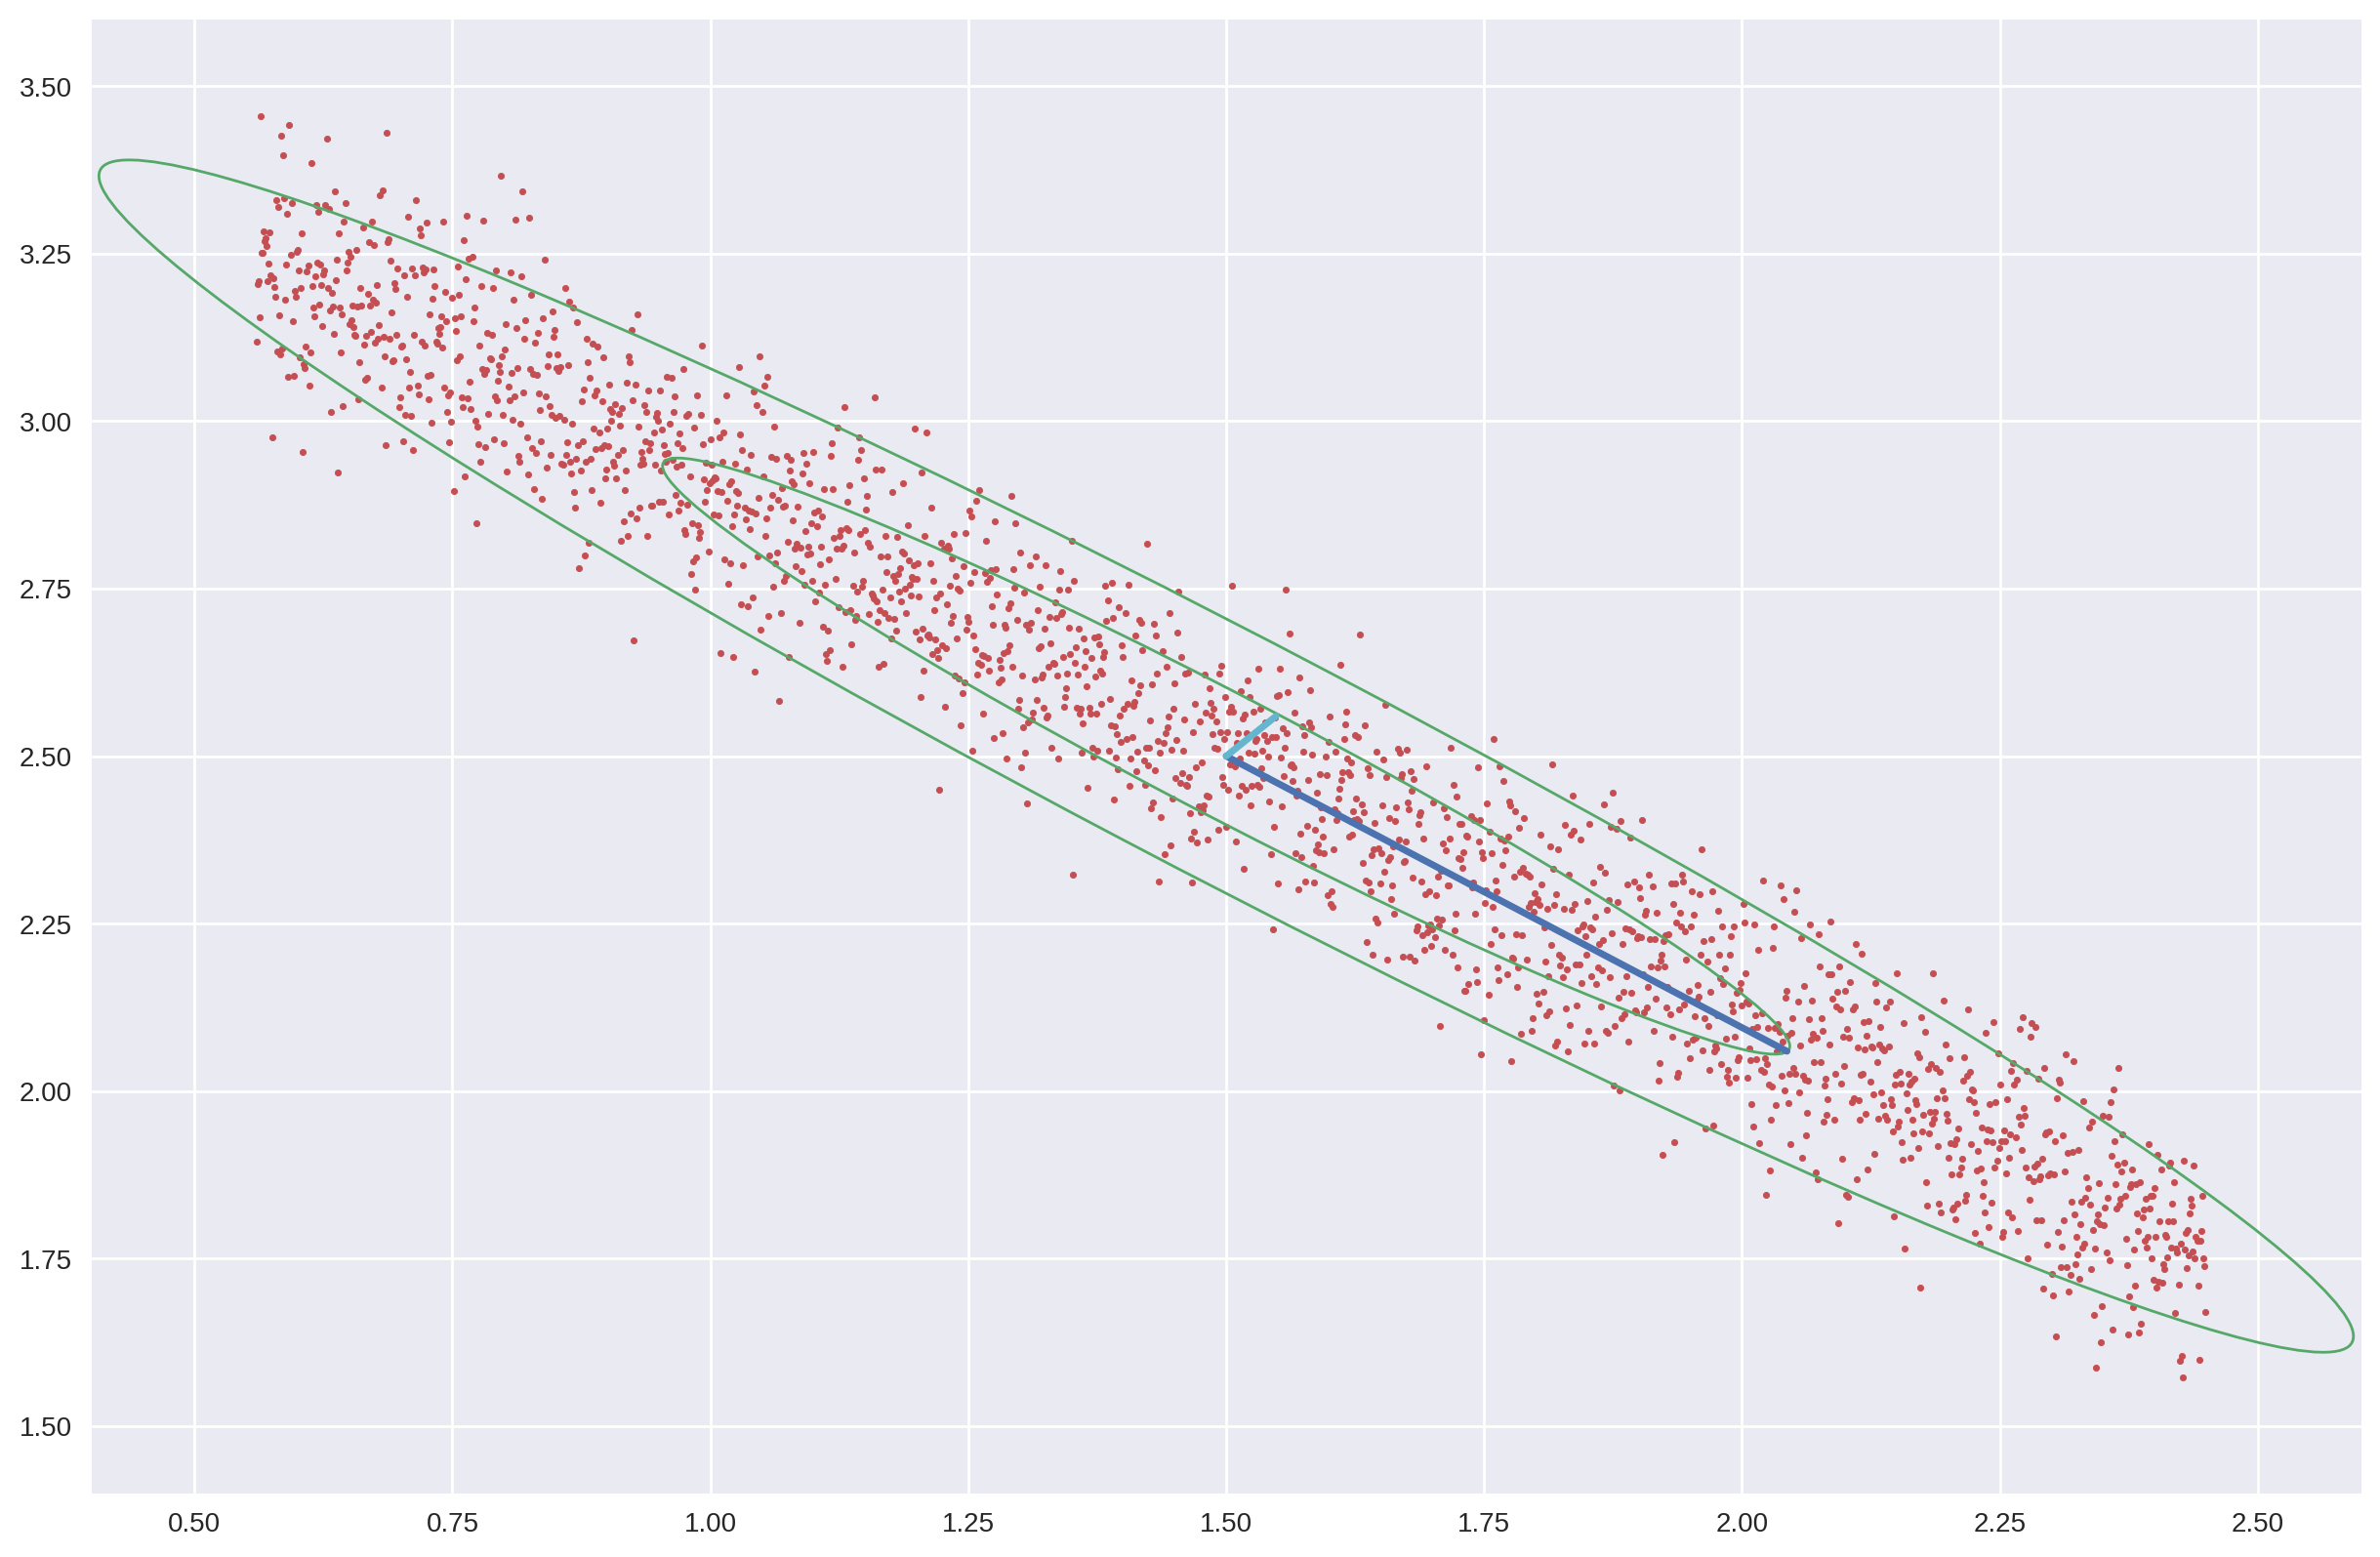
\includegraphics[width=\columnwidth]{PCA-Eigen_v2}
	\end{figure}
	
	\begin{figure}
		\begin{center}
			\caption{Histogram comparison of (a) classical and (b) PCA grayscale}
			\label{fig:hist}
			\includegraphics[width=\columnwidth]{lena_hist}\\
			\includegraphics[width=\columnwidth]{lena_pca_hist}
		\end{center}
	\end{figure}
	
	\begin{figure}
		\begin{center}
			\caption{Image-Comparison of non-PCA and PCA grayscale}
			\label{fig:lena_comp}
			\includegraphics[width=0.47\columnwidth]{lena_sw}
			\includegraphics[width=0.47\columnwidth]{lena_pca}
		\end{center}
	\end{figure}
	
	\subsubsection{correlation matrix}
	
	The correlation of input data can be visualized by the correlation matrix $R_{ij}$ stating how much feature $i$ is with feature $j$ correlated: $R_{ij} = \frac{Cov_{ij}}{\sqrt{Cov_{ii}\times Cov_{jj}}}$ ($Cov$ is the Covariance matrix of $\cal X$).
	
	A Value of $1$ means complete redundancy, a value of $-1$ means reciprocal redundancy and a value of $0$ means complete independence. Via plotting a histogram of this matrix we can get a quick overview of how much \emph{Lena} is correlated.
	
	\begin{figure}
		\caption{Pearson product-moment correlation coefficients between $0$ and $1$}
		\includegraphics[width=\columnwidth]{corrcoef}
	\end{figure}
	
	Thinking that everything is okay with \emph{Lena} is in this case wrong because the most values are below $0.3$ due to the fact that the upper left corner isn't much correlated with any value outside a range of 100 pixels. By looking into a certain region around the diagonal values, it's almost impossible to find values lower than $0.8$. But that's how an image works. There is a high probability that the pixels around a certain one have got an equally RGB-value.
	
	\subsubsection{PCA algorithm}
	
	Formally and according to \emph{Wikipedia} PCA is a statistical procedure using \textbf{orthogonal transformation} to convert a set of observations of possibly correlated variables into a set of values of linearly uncorrelated variables called \textbf{principal components}. It is defined in such a way that the first principal component has the \textbf{largest possible variance}, and each succeeding component, in turn, has the highest variance possible under the \textbf{constraint} that it is \textbf{orthogonal to the preceding components}.\\
	
	
	Algorithmically spoken we try to reduce data $X \color{gray}\in \mathbb{R}^{n\times m}$ from $n$-dimensions to $k$-dimensions by:
	\begin{itemize}
		\item mean normalization ($\mu = 0$, $\sigma = 1$)
		\item Compute covariance-matrix: $\Sigma {\color{gray}\in \mathbb{R}^{n\times n}} = \frac{1}{m}\sum_{i=1}^{n}(x^{(i)})(x^{(i)})^T = \frac{1}{m}X^T\times X$
		\item Compute eigenvectors $U \color{gray}\in \mathbb{R}^{n\times n}$ descending sorted by eigenvalues of matrix $\Sigma$: $[U, S, V] = svd(\Sigma)$
		\item Select the first $k$ eigenvectors from $U$: $Z {\color{gray} \in \mathbb{R}^{k\times m}} = U_{reduce}^T {\color{gray}\in \mathbb{R}^{n\times k}}\times X {\color{gray} \in \mathbb{R}^{n\times m}}$
		\item Variance retained (indicator of how much information we preserve): $\frac{\sum_{i=1}^{k}S_{ii}}{\sum_{i=1}^{n}S_{ii}}$; $S {\color{gray} \in \mathbb{R}^{n\times n}} = diag(eigvalues)$
	\end{itemize}
	
	\emph{Singular Value Decomposition (SVD)} offers us the ability to calculate eigenvectors and eigenvalues without assuming that the input matrix has to be a squared matrix. Since we only feed into the symmetric and squared Covariance matrix, this doesn't matter, but it's even more stable for singular covariance matrices, which could be a problem if one feature has always the same value.
	
	Generally spoken, because of the symmetric nature of the Covariance matrix, we get by the diagonalizing process $A = P\times D\times P^{-1}$ an orthogonal eigenvectors matrix $P$ and the diagonal eigenvalues matrix $D$. SVD states that $A = U\times S \times V$ whereas $U = P$ and $S = D$ so that the only difference towards the classical diagonalizing process is that we won't assume, that $P$ needs to be invertible.
	
	\subsubsection{Eigenfaces}
	
	"Labeled faces in the wild`` \emph{(LFW)} is a dataset by the University of Massachusetts~\cite{LFW} of $(X \in \mathbb{N}^{50\times 37})$ dimensional images of popular faces, which enables huge visualization opportunities according to the idea of~\cite{eigenfaces}. In \autoref{fig:eig_features} we get a visualization of the Top 12 eigenfaces being our new features when training a neural network for these \emph{LFW} dataset. For every eigenface there is a percentage available of how much information is in this particular eigenface. E.\,g. when using only the first eigenfaces we can retain almost $20\,\%$ of our original data, using $\nicefrac{5}{1850}$ of our data we retain $53\,\%$, $\nicefrac{20}{1850}$ retains $75\,\%$, $\nicefrac{185}{1850}$ retains $97\,\%$ and $\nicefrac{500}{1850}$ retains $99,7\,\%$.
	
	By simply reducing our data by the factor $10$ we are able to retain $97\,\%$ of our original image, which offers us the ability to train a lot faster and therefore compute more iteration giving us a better prediction. The loss of $3\,\%$ in the data is in this case negligible. Contrastive behavior can be observed if we reduce our data to $5$ dimension, where we are not able to differ between e.\,g. Bush and Blair, so training on these images would be useless if we want to predict the different persons.
	
	\begin{figure}
		\caption{Eigenfaces Original samples vs. Top 12 eigenface-features}
		\label{fig:eig_features}
		\begin{tikzpicture}
		\node[inner sep=0pt] (l) {\includegraphics[width=\columnwidth]{eigenface-orig}};
		\node[inner sep=0pt] (r) [below=of l] {\includegraphics[width=\columnwidth]{eigenface-pred}};
		
		\draw[thick,ForestGreen] (l.south) -- (r.north)
		node[midway,fill=white] {PCA};
		\end{tikzpicture}
	\end{figure}
	
	\begin{figure}
		\caption{Eigenfaces -- LFW: $\nicefrac{5}{1850}$ - $53\,\%$}
		\includegraphics[width=\columnwidth]{eigenface-5}
	\end{figure}
	\begin{figure}
		\caption{Eigenfaces -- LFW: $\nicefrac{20}{1850}$ - $75\,\%$}
		\includegraphics[width=\columnwidth]{eigenface-20}
	\end{figure}
	\begin{figure}
		\caption{Eigenfaces -- LFW: $\nicefrac{185}{1850}$ - $97\,\%$}
		\includegraphics[width=\columnwidth]{eigenface-185}
	\end{figure}
	\begin{figure}
		\caption{Eigenfaces -- LFW: $\nicefrac{500}{1850}$ - $99,7\,\%$}
		\includegraphics[width=\columnwidth]{eigenface-500}
	\end{figure}
	%http://vis-www.cs.umass.edu/lfw/
	
	\subsubsection{PCA for visualization}
	
	A last remark on PCA is about that it's also useful for visualization purposes in order to reduce very high dimensional data like e.\,g. the weights of our Neural Net trained towards the \emph{MNIST}-dataset describing ten-thousands of handwritten digits in dimension $28\times 28$ to 2D or 3D data in order to have the best view how to look on the dataset with the biggest variance, so you can see e.\,g. the predicted decision-boundary for the ten different digits and how good our network performs. Even for nun AI-purpose this visualization purpose is useful and takes advantages.
	
	\begin{figure}
		\caption{MNIST dataset~\cite{mnist}}
		\includegraphics[width=\columnwidth]{mnistv2}
	\end{figure}
	
	\begin{figure}
		\caption{PCA for Visualization -- Projecting on the best fitting (i.e. maximal variance) plane throughout the $784~dim$ space of the 10 different MNIST-digits}
		\includegraphics[width=\columnwidth]{TSNE_v2}
	\end{figure}
	
	\subsection{CNN}
	
	The last possible technique is to use a \emph{CNN}, which has got all those feature reductions and optimization stuff included. But this isn't a part of my seminar work.
	
	\section{Closing remarks}
	
	To sum up this overview of common optimization techniques we learned not only what they're about but also how to use them and at which time in your project it might useful to spend time towards certain optimization. We started with optimization in the model view with concrete \emph{Gradient Descent} alternatives like \emph{Momentum}, \emph{RMSProp} or \emph{ADAM}, going onwards to a very high-level \emph{Batch-Normalization} and ended up with \emph{Feature Optimization} emphasizing the importance of Data Analysis and Feature understanding.
	
	As long as you are a master in machine learning, most time you will spend on gathering data, analyzing data and simplifying data. Since algorithms are already written in thousands of deep learning framework like \emph{TensorFlow}, \emph{Keras}, etc, it'll be not that useful to invest your time on that stuff even when you are already familiar with common deep learning techniques. Backpropagation algorithms can nowadays implicit inferred by how you implement forward-propagation, so you won't bother about this error-prone task anymore.
	
	Even with techniques like \emph{transfer learning} or \emph{multi-task learning} you are able to use pre-trained weights and simply remove the last \emph{softmax}-prediction-layer on that network and feed in those high-level learning features on the pre-last layer in your own new and simpler neural network. E.\,g. \emph{YOLOv3} is a modern pre-trained CNN recognizing hundreds of different classes in images and videos. You can even use this network if you only want to predict traffic relevant objects like traffic lights/signs, cars, trucks, persons or bicycles by simply adding a logistic regression network on the end of \emph{YOLOv3}s pre-last layer. This enables dozens of new business cases without relying on good learnable data and the long-time learning process.
	
	\emph{End-to-End-Deep-Learning} in contrast is something you should forget. Most of the times the amount of data needed for modeling your overall task with one single and powerful model is not countable. But on the other hand, only relying on your project on non-AI software might be also not the best solution. The combination of algorithms and AI and a feasible pipeline is currently the best way. E.\,g. an end-to-end model of predicting cancer or non-cancer on medical data is not realizable due to the small amount of available data. But a pipeline like first removing the background and somehow pre-marked the important area with \emph{OpenCV} and afterward feeding this output to a neural net result in much higher prediction accuracy, because you ensure that the neural network is focused on the relevant data and doesn't get confused by wired-formed bones or other irrelevant data.
	
	\bibliography{refs}
	\bibliographystyle{plain}
	
	
	\listoffigures
	
\end{document}